\documentclass[12pt,a4paper,twoside,openany]{book}

%%%%%%%%%%%%%%%%%%%%%%%%%%%%%%%%%%%%%%%%%%%%%%%%%%%%%%%%%%%%%%%%%%%%%%%%
%%%%%%%% DULEZITE PRIKAZY, PRECTETE SI KOMENTARE A DOPLNTE JMENA %%%%%%%
%%%%%%%%%%%%%%%%%%%%%%%%%%%%%%%%%%%%%%%%%%%%%%%%%%%%%%%%%%%%%%%%%%%%%%%%

\usepackage{pdflscape}
\usepackage{subcaption}
\usepackage{xcolor}
\definecolor{comment}{rgb}{0, 0, 1} % comment barva
\newcommand{\comment}[1]{\textcolor{comment}{#1}}
\definecolor{purpose}{rgb}{0, 0.7, 0} % meaning barva
\newcommand{\purpose}[1]{\textcolor{purpose}{#1}}
\definecolor{source}{rgb}{1, 0, 0} % meaning barva
\newcommand{\source}[1]{\textcolor{source}{#1}}
\usepackage{graphicx}
\usepackage{tikz}
\usetikzlibrary{arrows.meta} % For better arrow tips
\usepackage{float} % Přidá mi H jako možnost ve figure místo hptb



% listings setup
\usepackage{listings}
\usepackage[czech]{babel}
\renewcommand{\lstlistingname}{Ukázka kódu} % Nastavení českého překladu

% JS jazykova definice a pozadi do listings
\definecolor{lightgray}{rgb}{.9,.9,.9}
\definecolor{darkgray}{rgb}{.4,.4,.4}
\definecolor{purple}{rgb}{0.65, 0.12, 0.82}
\lstdefinelanguage{JavaScript}{
  keywords={break, case, catch, continue, debugger, default, delete, do, else, false, finally, for, function, if, in, instanceof, new, null, return, switch, this, throw, true, try, typeof, var, void, while, with},
  morecomment=[l]{//},
  morecomment=[s]{/*}{*/},
  morestring=[b]',
  morestring=[b]",
  ndkeywords={class, export, boolean, throw, implements, import, this},
  keywordstyle=\color{blue}\bfseries,
  ndkeywordstyle=\color{darkgray}\bfseries,
  identifierstyle=\color{black},
  commentstyle=\color{purple}\ttfamily,
  stringstyle=\color{red}\ttfamily,
  sensitive=true
}

\lstset{
   language=JavaScript,
   backgroundcolor=\color{lightgray},
   extendedchars=true,
   basicstyle=\footnotesize\ttfamily,
   showstringspaces=false,
   showspaces=false,
   numbers=left,
   numberstyle=\footnotesize,
   numbersep=9pt,
   tabsize=2,
   breaklines=true,
   showtabs=false,
   captionpos=b
}





\input{settings/layout_commands.tex} % nacteni novych prikazu
\thesislanguage{czech} % prace bude v cestine, (diakritiku v nazvech sekci, kapitol, jmenu autora, nazvu prace atp. doporucuju psat pomoci specialnich znaku)
%\thesislanguage{english} % prace bude v anglictine

%\visualmode{print} % print mode - vhodne pro tisk, prazdne stranky na zacatku aby dulezite casti byly na liche strane, asymetricke okraje pro vazbu, cisla stranek v rozich
\visualmode{screen} % screen mode - vhodne pro elektronickou verzi, zadne prazdne stranky, symetricke okraje, cisla stranek uprostred



\thesisauthor{David Strašák} % jmeno autora prace, l
\thesissupervisor{Ing. Martin Formánek} % jmeno vedouciho
\thesistitle{Návrh systému pro dálkové spouštění dopravníků} % nazev prace


\input{settings/vut_style.tex} % nastaveni stylu dokumentu
%%%%%%%%%%%%%%%%%%%%%%%%%%%%%%%%%%%%%%%%%%%%%%%%%%%%%%%%%%%%%%%%%%%%%%%%

\usepackage{csquotes}
\usepackage[backend=biber,style=iso-numeric,sorting=none]{biblatex} % https://github.com/michal-h21/biblatex-iso690
\DeclareFieldFormat{labelnumberwidth}{\mkbibbrackets{#1}}
\addbibresource{chapters/bibtex_references.bib}



\begin{document}
	
%% titulni list + zadani - oba dokumenty lze stahnout ve studisu, zadani muzete naskenovat a prilozit podepsane (v PDF)
% \VUTtitle{introPages/TitulniList.pdf}{introPages/Zadani.pdf} % vlozi pdf do dokument
% \VUTtitle{pages/titulni_color.pdf}{blank} % vlozi prazdne misto pro originalni zadani a podepsanou kopii pri tisku (pouzit ve verzi print)


\abstract{ % abstrakt cesky
	...Abstrakt...
	}{ % abstrakt anglicky
	...anglicky...
	}{ % klicova slova česky
	...klíčová slova...
	}{ % klicova slova anglicky
	...anglicky...
    } % vyrobi i citaci

\acknowledgements{
	Prohlašuji, že předložená bakalářská práce je původní a zpracoval jsem ji samostatně. Prohlašuji, že citace použitých pramenů je úplná, že jsem ve své práci neporušil autorská práce (ve smyslu Zákona č. 121/2000 Sb., o právu autorském a o právech souvisejících s právem autorským).
	}{
    Tímto bych chtěl poděkovat všem, kteří se radou nebo jakoukoliv pomocí podíleli na vzniku této bakalářské práce. Především panu Ing. Martinu Formánkovi, za odborné vedení, odpovědi na mé dotazy a za cennou zpětnou vazbu při návrhu a tvoření této bakalářské práce. Velké díky za podporu také patří mé partnerce, rodině a všem přátelům.
    } % vlozi prohlaseni a podekovani


\vutpagestyle % prepise styl stranky, vlozi obsah

%%%%%%%%%%%%%%%%%%%%%%%%%%%%%%%%%%%%%%%%%%%%%%%%%%%%%%%%%%%%%%%%%%%%%%%%
%%%%%%%%%%%%%%%%%%%%% PROSTOR PRO KAPITOLY PRACE %%%%%%%%%%%%%%%%%%%%%%%
%%%%%%%%%%%%%%%%%%%%%%%%%%%%%%%%%%%%%%%%%%%%%%%%%%%%%%%%%%%%%%%%%%%%%%%%

% \chapter*{Úvod (co znamenají jednotlivé barvy v osnově plus)}\label{chap:uvod}\addcontentsline{toc}{chapter}{Úvod \textcolor{comment}{(co znamenají jednotlivé barvy v osnově plus)}}

\section*{Zde jsou vysvětlivky barev v textu:}

\comment{Modrou barvou jsou moje otázky na zkušenější akademiky - vedoucí nebo kdokoliv kdo tomu rozumí :)}

\purpose{Zelenou barvou jsou obecný popis o tom co v dané kapitole bude}

\source{Červenou barvou jsou informace o tom, kde seženu zdroje pro tuhle kapitolu. Budu rád když mi dáte vědět jestli jsou tyhle zdroje v pořádku, nebo ne.}

Černou barvou jsou moje myšlenky co souvisí s kapitolami - je to základ textu bakalářky bez nějaké větší editace (ale snažil jsem se aby dávaly smysl).

\section*{Co znamená ta suma za nadpisy}
$\sum$ znamená kolik stran předpokládám, že bude mít daná kapitola až bude napsaný všechen text práce. Je to počet i s obrázky. Obrázků tolik není takže se nebojím že bych měl málo textu.

\section*{Názvy kapitol}
Názvy kapitol jsou teď jenom nastřelené a nejspíš nezní dobře. Snažil jsem se spíš aby reflektovaly myšlenku kapitoly.
% Co udělal někdo jinej
\chapter{Rešerše} \label{chap:Rešerše}
\section{Frekvenční měniče a jejich role v řízení dopravníků}\label{sec:FrekvencniMeniceAJejichRole}
%\purpose{Vysvětlit s jakým systémem už pracuji}

Dopravníkové systémy byly kdysi pouze robustní mechanické konstrukce s jednoduchým asynchronním motorem napojený na jednu hodnotu síťového napětí a s nemotornou regulací rychlosti například pomocí přidáním odporu do sekundárního vinutí. V dnešní době jsme v éře průmyslu 4.0. a s tím je v každém mechatronickém systému důraz na automatizaci a digitalizaci spojených procesů. Díky velkému pokroku v oblasti výkonové elektrotechniky a řídících systémů vznikly nové možnosti precizního řízení otáček asynchronních motorů. Důležitým prvkem této transformace se staly frekvenční měniče - zařízení které umí na vstupu brát síťové napětí a na výstupu poskytovat jinou amplitudu a frekvenci napětí, což umožňuje efektivně řídit otáčky jakýchkoliv asynchronních motorů. Tohle umožnilo vznik dopravníkových systémů u kterých je možné přesně a efektivně řídit otáčky. Když se k tomuto systému přidají ještě řídící systémy, je možné znát v každé chvíli polohu balíků na lince a inteligentně tento tok balíků řídit.

Dopravníkové systémy, které společnost Honeywell vytváří jsou přesně takové inteligentní dopravníkové systémy. Cílem těchto systémů je pro zákazníky (většinou dopravní společnosti nebo například supermarkety) vytvořit systém, na který stačí vložit balík na jednom místě a tento balík už doputuje na místo kde má skončit. Řídící systém se postará o zbytek činností jako je třeba naskenování QR kódu na balíku, identifikace koncového bodu a řízení všech linek tak, aby nedošlo ke kolizím nebo nebezpečným událostem.

V současné době jsou tyhle jednotlivé dopravníky poháněné třífázovými asynchronními motory, které pomocí složitých převodů roztáčí celý dopravník (všechny jeho válečky nebo pás). Tyhle asynchronní motory jsou poháněné frekvenčními měniči a ty jsou pro většinu Honeywell dopravníkových systémů v dnešní době model G120D od značky Sinamics. Frekvenční měnič poskytuje výstup do asynchronního motoru, ale jedná se pouze o výkonovou část. Aby bylo možné frekvenční měnič řídit, je potřeba na něj připojit i ovládací panel, které je v běžné sestavě Honeywell dopravníkových systémů model CU240D-2 od značky Sinamics. Při běžném provozu je na tenhle ovládací panel připojená komunikační sběrnice PROFINET, která dává frekvenčnímu měniči ovládací příkazy. PROFINET je naprogramovaný přes Siemens TIA Portal (Total Integrated Automation Portal), což je prostředí vyvinuté od Siemens právě pro řízení různých frekvenčních měničů pomocí Siemens programovatelných logických automatů (PLC). V tomto programu je modelovaný tok na lince a pomocí toho PLC automaticky řídí dopravníkový systém.
\cite{SinamicsG120D}

Zařízení, které v je v této bakalářské práci navrženo se ale nekoncipuje pro standardní provoz dopravníkových systémů, protože tam je systém už řízený PLC. Tento systém je navrhovaný pro zjednodušení procesu kontroly kvality instalace a funkčnosti dopravníků, který je konaný hned po instalaci dopravníků (které instaluje externí firma) v prostorách zákazníků. Jedná se hlavně o dynamické kontroly kvality mechanické instalace, kdy se na každém dopravníku musí zkontrolovat, že je schopný pohybu bez přílišného házení nebo vibrací kvůli špatné instalaci.

V kontextu těchto zkoušek není nezbytné, aby frekvenční měniče komunikovaly prostřednictvím řídicího systému Siemens PLC. Opak je pravdou - zde je inicializace PLC sítě mezi dopravníky spíše extra úkol, což jsou schopnosti které často zaměstnanci kontrolující mechanickou instalaci dopravníků nemají. Při těchto zkouškách se stává prioritní mít kontrolu nad individuálními dopravníky a mít možnost je ovládat a nastavovat na nich rychlost dle libosti. Výhodou by zde při takovém ovládání byla i možnost implementace dálkového ovládání dopravníků.

\subsection{Jak frekvenční měniče fungují}\label{sec:JakFungujiFrekvencniMenice}
%\purpose{Vysvětlit jak vlastně ten frekvenční měnič funguje a proč ho používáme v dopravnících}

Jak již bylo naznačeno v kapitole \ref{sec:FrekvencniMeniceAJejichRole}, frekvenční měniče se pro řízení asynchronních motorů teoreticky používat nemusí, ale poté by měl dopravník jenom omezený výběr z nastavitelných rychlostí a celé řízení by bylo mnohem složitější. V dnešní době jsou frekvenční měniče technicky nejvýhodnější způsob regulace motorů jak z hlediska technických parametrů (regulační rozsah a přesnost), tak i z energetického hlediska (regulace je bezeztrátová). Kvůli těmto důvodům jsou frekvenční měniče tak časté.  \cite{FrekvencniMeniceZeSkriptElektrickeRegulovanePohony}

Frekvenční měnič Sinamics G120D je sice vektorově řízený, ale princip funkce frekvenčního měniče se dá lépe vysvětlit na měniči se skalárním řízením.

Rozdíl mezi těmito dvěma způsoby řízení spočívá v efektivitě. Vektorové řízení cíleně reguluje proud v cívkách asynchronního motoru tak, aby statorové magnetické pole bylo prostorově optimálně natočené vůči poli rotorovému (úhel závisí na počtu pólů). Díky tomu je dosaženo efektivnějšího pohonu rotoru požadovanou rychlostí a směrem. Skalární řízení naopak tento vzájemný úhel nesleduje, a proto není z hlediska řízení optimální. Vektorové řízení je zkrátka složitější, ale efektivnější a má další výhodu že umožňuje přímé řízení momentu.
\cite{FrekvencniMeniceZeSkriptElektrickeRegulovanePohony}

Funkce frekvenčního měniče vychází přímo z principu funkce asynchronního motoru. Při návrhu asynchronního motoru se navrhuje velikost sycení motoru které je určeno spřaženým magnetickým tokem statorového vinutí $\Psi_S$ který je definován jako:
\begin{equation}
	\Psi_S = N\Phi_S
	\label{eq:SdruzenyMagnetickyTok}
\end{equation}
kde N je počet závitů cívky na statoru a $\Phi_S$ je magnetický tok jednoho závitu cívky.

Aby frekvenční měnič mohl fungovat, musí být spřažený magnetický tok statorového vinutí konstantní. Tomu se říká \textbf{Podmínka konstantního sycení}. Statorové vinutí motoru je napájeno nějakým harmonickým napětím vycházející z frekvenčního měniče o tvaru:
\begin{equation}
	U_S(t) = U_{max}sin(\omega_st)
	\label{eq:NapetiNaStatoru}
\end{equation}
kde $U_S$ je napětí na statoru, $U_{max}$ je amplituda statorového napětí a $\omega_s$ je úhlová frekvence napájecího napětí.
\cite{SkriptaRizeniOtacekAM}

Pokud zanedbáme statorový odpor a budeme tedy uvažovat, že celé statorové napětí $u_L$ bude na indukčnosti motoru, bude maximum spřaženého magnetického toku ve statoru rovné: \cite{SkriptaRizeniOtacekAM}
\begin{equation}
	\Psi_S = \int_0^{T/2} u_L \, dt
	\label{eq:PodminkaKonstantnihoSyceni}
\end{equation}


Princip podmínky konstantního sycení tedy spočívá v tom, že chceme mít konstantní spřažený magnetický tok. Tohle se dělá z důvodu, že na sycení motoru závisí například magnetizační proudy. Křivka sycení není lineární a má bod zvratu, kdy se menší změna sycení projeví ve mnohem větším zvýšení magnetizačního proudu než tomu bylo před bodem zvratu. Konstantní sycení je nastaveno proto, abychom zůstali před bodem zvratu a díky tomu bude magnetizační proud růst pomaleji a rozumně.

\subsubsection{Režimy funkce frekvenčního měniče}
Asynchronní motor, který je napájen z frekvenčního měniče má dva provozní režimy ve kterých se může nacházet. Těmi jsou oblast konstantního momentu a oblast konstantního výkonu zobrazené v grafu \ref{fig:provoznirezimyamsfrekvencnimmenicem}.

\begin{figure}[hptb]
	\centering
	\includegraphics[width=1\linewidth]{images/ProvozniRezimyAMSFrekvencnimMenicem}
	\caption{Závislost napětí, momentu a výkonu na frekvenci \cite{SkriptaRizeniOtacekAM}}
	\label{fig:provoznirezimyamsfrekvencnimmenicem}
\end{figure}

V levé části grafu je oblast konstantního momentu s plným sycením motoru. Zde platí podmínka definovaná v rovnici \ref{eq:PodminkaKonstantnihoSyceni} o konstantním spřaženém magnetickém toku ve statoru. Díky tomu je moment na motoru konstantní a postupně motoru roste výkon, který je definovaný jako:
\begin{equation}
	P = M\omega
	\label{eq:vykonmotoru}
\end{equation}
až do maximální hodnoty výkonu která je v bodě $n$ - jmenovitý bod motoru.

Je také dobré podotknout, že levá část grafu nemůže jít takto od nulového napětí (tento graf je spíše idealizovaný případ), ale jde zpravidla od 10\% jmenovité hodnoty napětí, jelikož se musí pokrýt ztráty které vznikají na odporu statorového vinutí $R_S$. \cite{SkriptaRizeniOtacekAM}

V pravé části grafu je oblast konstantního výkonu ve kterém se motor odbuzuje. Zde už není splněna podmínka z rovnice \ref{eq:PodminkaKonstantnihoSyceni} a tak motoru klesá moment. Vzhledem k tomu, že frekvence statorového napětí stále roste, tak rostou stále i otáčky rotoru.

\subsection{Sinamics G120D}
%\purpose{Popsat hlavní parametry frekvenčního měniče - rozsah napájecího napětí, maximální proud, podporovaný komunikační protokoly (Profinet) - nějaký basic info o Sinamics G120D. Tady přidat i to že Sinamics G120D pracuje s asynchronními motory - jaké jsou od Siemens třeba nejčastější?}

Sinamics G120D je decentralizovaný frekvenční měnič designovaný pro buzení motorů od dopravníkových systémů po elektrické monoraily. Slovo decentralizovaný zde znamená, že frekvenční měnič není jeden centralizovaný, ale že je víc menších frekvenčních měničů blízko u motorů, které ovládají. Kvůli tomu má i certifikaci IP65, která zaručuje dostatečnou kvalitu zpracování, aby bylo možné mít tento frekvenční měnič v náročných prostředí skladů zákazníků firmy Honeywell.
\cite{SinamicsG120D}

Frekvenční měnič obsahuje funkce jako je přesné nastavení polohy motoru, bezpečnostní funkce a dobře konfigurovatelné digitální a analogové vstupy a výstupy. Je to standardní frekvenční měnič který je používán v různých aplikacích hlavně firmami které fungují jako systémoví integrátoři. Běžná podoba tohoto frekvenčního měniče (s kontrolním panelem CU240D-2) je na obrázku \ref{fig:sinamics_G120D}.
\cite{SinamicsG120D}

\begin{figure}[hptb]
	\centering
	\includegraphics[width=0.8\linewidth]{images/Sinamics_G120D.png}
	\caption{Frekvenční měnič Sinamics G120D \cite{SinamicsG120D}}
	\label{fig:sinamics_G120D}
\end{figure}

Sinamics G120D se v rámci systémů společnosti Siemens dá používat s třífázovými asynchronními motory řad Simotics GP (General Purpose) a Simotics SD (Severe Duty). Jak už název napovídá tak v případě společnosti Honeywell je jako motor nejčastěji používán Simotics GP. Napájecí napětí frekvenčního měniče je také třífázové od $380V$ do  $500V$ dle konfigurace motoru a frekvenční měniče se vyrábí s výkonem $0,75kW$ až $7,5kW$.

Tento frekvenční měnič je tvořen dvěma hlavními částmi - výkonová část a ovládací panel. Ovládací panel ovládá a monitoruje výkonovou část frekvenčního měniče pomocí několika kontrolních systémů na bází uzavřených smyček a díky tomu může kontrolovat bezpečný stav frekvenčního měniče a taky znemožnit ovládání, pokud by s měničem bylo něco v nepořádku. Také je schopný rekuperace energie z brždění linek a vracet ji do sítě, což zákazníkům snižuje náklady na provoz.
\cite{SinamicsG120D}

Všechny tyto funkcionality je možné ovládat přes průmyslové sběrnice PROFINET, PROFIBUS anebo běžnou sběrnicí EtherNet. Tímto způsobem dává PLC příkazy frekvenčnímu měniči v běžném režimu ovládání dopravníků.

\subsection{Nastavení ovládacího panelu}\label{sec:NastaveniOvladacihoPanelu}
%\purpose{Vysvětlit jak se dají dopravníky nastavit aby fungovaly s mým systémem}

Jak bylo dříve zmíněné frekvenční měnič má vždy nějaký ovládací panel. V případě Honeywell instalací je ovládací panel většinou typu Sinamics CU240D-2. Ovládací panely tohoto typu lze za chodu seřizovat třemi způsoby (zobrazené i v obrázku \ref{fig:cu240comissioning}):
\begin{itemize}
	\item Připojení USB z notebooku
	\item Použití PROFINET nebo PROFIBUS
	\item Použití zařízení IOP-2 Handheld
\end{itemize}

\begin{figure}[hptb]
	\centering
	\includegraphics[width=0.7\linewidth]{images/CU240comissioning}
	\caption{Způsoby seřizování ovládacího panelu frekvenčního měniče \cite{SiemensG120DGettingStarted}}
	\label{fig:cu240comissioning}
\end{figure}

Vzhledem k předpokladu, že navrhovaný systém mají používat osoby, které nejsou inženýři specializovaní na kontrolní systémy, je nejvhodnější způsob jak seřizovat ovládací panel použít zařízení IOP-2 Handheld. Ostatní dvě metody vyžadují specializovaný software pro který by bylo zapotřebí instalovat a udržovat si pro něj licence. Naproti tomu IOP-2 Handheld představuje samostatné zařízení schopné provést veškerá potřebná nastavení a je dodáváno s optickým kabelem pro přímé připojení k ovládacímu panelu.

Pro účely navrhovaného systému je potřeba ovládací panel vyresetovat a nastavit do jednoho z  možných výchozích nastavení. Zvolené výchozí nastavení ovlivňuje celý systém, protože ten ovládá dopravník tím, že pomocí relé spíná digitální vstupy ovládacího panelu frekvenčního měniče - tímto způsobem dává systém příkazy na spuštění dopravníku, zrychlení a zpomalení. Nesprávné nastavení ovládacího panelu by vedlo k tomu, že ačkoliv by systém generoval správné signály na digitálních vstupech, panel by je interpretoval chybně.

Navržený systém je optimalizován pro výchozí nastavení číslo 9, ve kterém jsou funkce digitálních vstupů definovány tímto způsobem:
\begin{itemize}
	\item Digitální vstup 0: ON/OFF dopravníku
	\item Digitální vstup 1: Zrychlení dopravníku
	\item Digitální vstup 2: Zpomalení dopravníku
	\item Digitální vstup 3: Kvitování chyby
\end{itemize}
Systém bude konektory připojený k ovládacímu panelu a pomocí relé na desce plošných spojů bude ovládat dopravník rozpojování a zkratováním těchto digitálních vstupů. Digitální vstup č. 3 nebude v rámci systému využíván, protože kvitování případných chyb je vyžadováno pouze jednorázově při resetování do výchozích nastavení a lze jej provést přímo pomocí zařízení IOP-2 Handheld.
\cite{SiemensG120DGettingStarted}.

Resetování ovládacího panelu do tohoto výchozího nastavení je možné provést přímo na místě pomocí zařízení Sinamics IOP-2 Handheld. Pro resetování stačí pouze připojit IOP-2 k ovládacímu panelu frekvenčního měniče, vybrat možnost pro zresetování nastavení ovládacího panelu a vybrat výchozí nastavení číslo 9. Zbytek hodnot na ovládacím panelu, jako je například zrychlující rampa, může zůstat na výchozích hodnotách, protože je není potřeba v rámci testování kvality instalace mít na správných hodnotách (frekvenční měnič funguje i tak). Poté je možné odpojit IOP-2 od ovládacího panelu, který tímto způsobem zůstane nastavený nadále.



\subsubsection{Alternativní výchozí nastavení ovládacího panelu}
%\purpose{popsat nastavení default with potentiometer a default MOP with E-STOP}

Při návrhu systému byla kromě výchozího nastavení číslo 9 zvažována i další relevantní výchozí nastavení, konkrétně nastavení č. 8 a č. 12.

Výchozí nastavení č. 8 by definovalo chování systému následovně:
\begin{itemize}
	\item Digitální vstup 0: ON/OFF dopravníku
	\item Digitální vstup 1: Zrychlení dopravníku
	\item Digitální vstup 2: Zpomalení dopravníku
	\item Digitální vstup 3: Kvitování chyby
	\item Digitální vstup 4: Při přerušení nouzově zastaví (E-STOP)
	\item Digitální vstup 5: Při přerušení nouzově zastaví (E-STOP)
\end{itemize}
Tohle výchozí nastavení nabízí stejnou funkcionalitu jako zvolené nastavení č. 9, ale vyžaduje připojení dalšího kabelu na kterém bude v obvodu umístěné bezpečnostní tlačítko E-STOP, které by také muselo mít dostatek místa ve schránce systému. Tohle výchozí nastavení bylo zamítnuto právě kvůli tomu, že E-STOP tlačítko vyžaduje neúměrně příliš mnoho místa a tak by to výrazně zvětšilo rozměry systému, což by zmenšovalo přenositelnost a jednoduchost používání. Bezpečnost systému je přitom zajištěna jinými bezpečnostními prvky přímo u dopravníků, jak je podrobněji popsáno v kapitole \ref{sec:PosouzeniZHlediskaBezpecnosti}.
\cite{SiemensG120DGettingStarted}

Další zvažovanou alternativou bylo výchozí nastavení č. 12, které by definovalo funkce vstupů tímto způsobem:
\begin{itemize}
	\item Digitální vstup 0: ON/OFF dopravníku
	\item Digitální vstup 1: Reverzace směru otáčení
	\item Digitální vstup 2: Kvitování chyby
	\item Analogový vstup: Nastavení rychlosti
\end{itemize}
Tohle nastavení by umožnilo připojení potenciometru k analogovému vstupu ovládacího panelu pro přímé nastavení rychlosti. Díky tomuto by bylo o jedno tlačítko méně na schránce systému, ale zároveň by to vyžadovalo speciální kabely pro připojení (vzhledem k tomu, že se analogové vstupy ovládacích panelů v instalacích Honeywell běžně nevyužívají) a také by to zahrnovalo modifikaci desky plošných spojů, například s využitím integrovaného obvodu digitálně řízeného potenciometru.
\cite{SiemensG120DGettingStarted}

Po zhodnocení těchto možností bylo vybráno výchozí nastavení č. 9.

\subsection{Bezpečnostní aspekty práce s ovládacím panelem}
%\purpose{Zmínit že když pracuji s takovýmto výkonovým zařízením, musím si dát pozor na bezpečnost. Vysoký napětí který vystupuje z frekvenčního měniče se dá vypnout přepínačem který je umístěný nad ovládacím panelem. Potom už člověk pracuje jen s 24V které jsou na všech portech ovládacího panelu a kvůli tomu všechny porty zakrývají šroubovací gumové kryty, které je potřeba oddělat předtím než se můžou připoji kabely ze systému co navrhuji.}

Vzhledem k tomu, že frekvenční měnič pracuje ve výkonové části s usměrněným trojfázovým napětím, je velmi důležité dbát na bezpečnost při práci s frekvenčním měničem. Z tohoto důvodu je vedle každé instalace frekvenčního měniče v Honeywell umístěn bezpečnostní vypínač, který vypojuje napájení výkonové části frekvenčního měniče. Pro bezpečné zacházení s frekvenčním měničem je potřebné mít tento vypínač ve stavu rozpojeno.

Po rozpojení napájení výkonové části zůstává na ovládacím panelu napětí $24V$. Tohle nízké napětí je ale chráněno šroubovacími gumovými krytkami, které zakrývají veškeré digitální vstupy a výstupy ovládacího panelu kde se toto napětí nachází.

\section{Open-source vývojové desky}
%\purpose{Zde bude úvod do open source vývojových desek.}

Mikrokontroller, mozek praktické části bakalářské práce, není integrován přímo na desce s výkonovou částí zařízení. Využita byla možnost open-source vývojové desky, přičemž toto označení je dnes často synonymem pro Arduino, značku s největším přínosem v této oblasti.

Myšlenka vývojových desek jako jsou Arduino desky začala myšlenkou minimalismu - desky nebyly nikdy převratné, ale obsahovaly přesně to, co je potřeba. Na jedné vývojové desce je obsažený mikrokontroller, převodník z USB do sériové komunikace a dle desky obsahuje další užitečné součástky. Je zde možné tedy nejenom využívat periferie použitého mikrokontrolleru, ale i další hardware, jako jsou externí krystaly, napájení mimo USB kabel a další na základě specifického návrhu vývojové desky.
\cite{KnihaOArduinu}

Rychlou adaptaci veřejností umožnil nejenom kvalitní design desek, ale i software pro programování Arduino desek na počítači. Na rozdíl od předchozího proprietárního softwaru, který nebyl dostupný pro všechny operační systémy, je programovací prostředí Arduina open-source a spustitelné na všech systémech s podporou Java aplikací.
\cite{KnihaOArduinu}

Kromě výhod ekosystému Arduino existují obecné důvody pro použití hotových vývojových desek namísto přímé integrace mikrokontrolleru v prototypování a vývoji. Mezi hlavní výhody patří možnost připojení vývojové desky pomocí kolíkových lišt, což umožňuje snadné vyjmutí pro přeprogramování nebo výměnu. Přímá integrace by v případě poruchy vyžadovala odpájení. Díky tomu vývojová deska celkově usnadňuje prototypování a opravitelnost.

Nakonec je důvodem zvolení open source vývojových desek do systému i jejich dostupnost a flexibilita kterou nabízejí. Jelikož jsou schémata zapojení desek veřejně dostupná, může je vyrábět jakýkoliv výrobce. Navíc je také možné používat veřejně dostupná schémata zapojení desek při návrhu vlastních desek plošných spojů do kterých jsou vývojové desky integrované a díky tomu známá přesná propojení jednotlivých komponentů v celé navržené desce plošných spojů.

\subsection{Proč WEMOS vývojové desky}
%\purpose{Tady bude popsané co jsou WEMOS desky a proč je používám. Taky tady bude důvod proč jsem si vybral WEMOS D1 Mini pro a srovnání s wemos D1 mini a arduino UNO}

Arduino v dnešní době není jediná firma, která vyrábí open-source vývojové desky. Pro tuhle bakalářskou práci byla zvolena vývojová deska od společnosti WEMOS, která je výrobce vývojových desek které jsou podobné Arduino deskám, ale jejich zaměření je specificky ve vytváření kompaktních desek které mají integrovanou bezdrátovou konektivitu (WiFi a bluetooth) pomocí populárních mikrokontrolérů ESP32 a ESP8266 od společnosti Espressif Systems.

Mít možnost používat WiFi je důležitý požadavek, který musí vývojová deska splňovat. Pokud bude systém možné ovládat přes WiFi, je možné pro ovládání použít jakékoliv zařízení, které má WiFi technologii, což je v dnešní době většina chytrých zařízení. Kvůli tomu lze dopravník ovládat širokým spektrem chytrých zařízení a tak není potřeba aby s sebou uživatelé nosili dedikovaný vysílač.

Společnost WEMOS nabízí několik modelů vývojových desek s různými mikrokontroléry a periferiemi. Mezi známé varianty patří například:
\begin{itemize}
	\item \textbf{WEMOS D1 Mini:} Kompaktní deska postavená na mikrokontroléru ESP8266EX. Poskytuje 11 digitálních GPIO pinů (z toho 10] s podporou PWM a podporou přerušení), 1 analogový vstup, I2C rozhraní, 4MB Flash paměti a integrovanou PCB anténu pro WiFi. Napájení a programování se provádí přes USB-C konektor. Deska je oblíbená pro své malé rozměry a širokou podporu, ale omezuje ji malý počet GPIO pinů, což desku nedělá dobrou pro prototypování nebo rozsáhlejší aplikace.
	\item \textbf{WEMOS C3 Mini:} Novější varianta využívající mikrokontrolér ESP32-C3. Tento čip integruje WiFi i Bluetooth konektivitu. Deska disponuje USB-C konektorem, 4 MB Flash paměti a 12 GPIO pinů.
\end{itemize}

Tenhle systém je ale navrhován pro industriální prostředí a je velmi důležité aby byla bezdrátová komunikace co nejspolehlivější. Proto je potřebné mít na vývojové desce k dispozici externí anténu, která významně zvýší dosah WiFi komunikace díky lepšímu umístění antény. Proto byla do systému vybrána vývojová deska WEMOS D1 Mini Pro kterou lze vidět na obrázku \ref{fig:WEMOSD1MiniPro}. Tato deska sdílí většinu vlastností s modelem D1 Mini, ale narozdíl od levnějšího modelu má 16MB Flash paměti, které jsou také velmi důležité vzhledem k tomu, že na kód pro systém by 4MB Flash paměti nestačilo.

Všechny vývojové desky WEMOS s mikrokontroléry ESP8266 a EPS32 lze programovat pomocí prostředí Arduino IDE (nebo alternativy jako PlatformIO) s využitím Arduino jazyka založeného na C++, nebo alternativně pomocí MicroPython. Celá aplikace je programována pomocí Arduino framework pro ESP8266. Webové ovládání je prováděno pomocí knihovny WebServer, která umožňuje běh nenáročných síťových aplikací (více je popsané v kapitole \ref{sec:ArduinoFrameworkForESP8266}).

\begin{figure}[hptb]
	\centering
	\includegraphics[width=0.8\linewidth]{images/WEMOS_D1_Mini_Pro.png}
	\caption{Použitá varianta vývojové desky WEMOS D1 Mini Pro \cite{WEMOSD1MiniPro}}
	\label{fig:WEMOSD1MiniPro}
\end{figure}

\subsection{Technické specifikace WEMOS D1 Mini Pro}
% \purpose{Rozvinout co jsou specifikace D1 Mini Pro a co ty jednotlivé věci znamenají - počet GPIO, I2C, PWM, paměť, typ mikrokontrolleru, atd. - nějaký základní basic informace}

Na základě požadavků projektu a srovnání s alternativami je pro realizaci hardwarového návrhu nejefektivnější vývojová deska WEMOS D1 Mini Pro. Tato sekce popisuje její technické parametry s jejich využitím v návrhu. Samotná deska je postavena na mikrokontroléru ESP-8266EX a je velmi kompaktní, zatímco ale stále poskytuje dost funkcionalit a vstupních a výstupních pinů pro provoz zařízení.

Technické specifikace této vývojové desky jsou následující: \cite{ESP8266EXDatasheet, D1MiniProDokumentace}
\begin{itemize}
	\item Mikrokontrolér: ESP-8266EX
	\item Napájecí napětí: $5V$
	\item Provozní napětí: $3,3V$
	\item Počet digitálních I/O pinů (GPIO): 11. Tyto piny slouží pro digitální vstupní a výstupní signály které budou ovládat dopravník a na základě kterých se bude aproximovat rychlost dopravníku.
	\item Podpora periferií na GPIO pinech: Většina digitálních pinů podporuje funkce jako:
	\begin{itemize}
		\item Přerušení (Interrupt): Umožňuje reakci mikrokontroléru na externí události.
		\item PWM (Pulse Width Modulation): Pro generování semi-analogového signálu nebo snížení střední hodnoty napětí. Až 10 pinů má podporu PWM.
		\item I2C: Dvouvodičová sériová sběrnice používaná pro komunikaci s periferiemi, jako je v tomto projektu použitý LCD displej. Deska disponuje dedikovanými piny pro tuto sběrnici na pinech D1 a D2.
		\item One-wire: Sériová sběrnice pro komunikaci s některými typy senzorů.
	\end{itemize}
	\item Analogový vstupní pin: 1. Tento pin umožňuje měřit analogové napětí, například z některých typů senzorů. Maximální vstupní napětí pro tento pin je 3.2V.
	\item Paměť:
	\begin{itemize}
		\item Flash paměť: 16 MB. Tato velká kapacita Flash paměti je důležitá pro uložení aplikačního kódu, rozšiřujících knihoven (jako je WebServer) a webových souborů co jsou hostované na serveru.
		\item RAM: 50 kB. Slouží pro běh programu a ukládání proměnných.
	\end{itemize}
	\item Bezdrátová konektivita: Integrovaná WiFi na frekvenci 2.4 GHz.
	\item Anténa: Možnost připojení externí antény prostřednictvím IPEX1 / SMA konektoru nebo využití vestavěné keramické antény pro testování. Pro zvýšení spolehlivosti a dosahu v industriálním prostředí je využita možnost externí antény.
	\item Napájení a programování: Micro USB konektor. Deska může být napájena přes USB nebo přes 5V pin.
	\item Napájení z baterie: Rozhraní pro připojení lithiové baterie s nabíjecím proudem až 500mA. Toto rozhraní ale v tomto projektu není využíváno a navržená deska plošných spojů není pro používání baterie uspořádána.
	\item Kompatibilita: Deska je kompatibilní s vývojovými prostředími a firmwary jako Arduino, MicroPython a NodeMCU, což poskytuje flexibilitu při vývoji firmwaru.
\end{itemize}

Zapojení vývojové desky do navrhnuté desky plošných spojů je popsáno v kapitole \ref{sec:Hardware}.

\subsection{Arduino framework pro ESP8266}\label{sec:ArduinoFrameworkForESP8266}
% \purpose{Trochu uvést do kontextu jak funguje arduino framework for esp8266 a jak specificky řeším provozování webserveru na mým MCU.}

Pro programování mikrokontrolerů z řad EPS8266 je možné využít jejich nativního software development kitu (SDK) anebo takzvaný "Arduino framework" pro tuto platformu. Tato knihovna je portace SDK pro platformu Arduino a díky tomu je možné používat prostředí jako je Arduino IDE nebo Platformio pro programování ESP8266 mikrokontrolerů. Tohle všechno je možné i přesto, že mají ESP8266 i Arduino přirozeně různé základy, které spolu ve výchozím stavu nejsou kompatibilní. Tato podpora umožňuje velkému množství hobby i profesionálním programátorům programovat ESP8266 mikrokontrolery ve stejném prostředí jako ve kterém programovali své Arduino projekty. To všechno bez ztráty hardwarových nebo síťových periferií.

"Arduino framework pro ESP8266 je podpora ESP8266 mikrokontroleru pro Arduino prostředí. To vývojářům umožňuje používat známé Arduino funkce a knihovny, které je možné spouštět přímo na ESP8266 mikrokontrolleru." \cite{ESP8266ArduinoFrameworkGithub}

V této práci byl kód mikrokontroleru programován uvnitř programovacího prostředí PlatformIO (ukázané na obrázku \ref{fig:PlatformioUkazka}) ve kterém byl Arduino framework pro ESP8266 využitý. Byla využitá i kompatibilita s existujícími Arduino knihovnami, jako v případě knihovny Ticker. To je knihovna, která v rámci Arduino zařízení umožňuje nastavit časovač, který spouští některou funkci pravidelně přesné časové intervaly.

\begin{figure}[hptb]
    \centering
    \includegraphics[width=0.9\linewidth]{images/Platformio_Ukazka.png}
    \caption{Ukázka rozhraní vývojového prostředí Platformio}
    \label{fig:PlatformioUkazka}
\end{figure}

\subsubsection{Knihovny pro webové funkce}
%\purpose{Popsat co dělají knihovny ESP8266WiFi, WiFiClient, ESP8266WebServer a ESP8266mDNS}

Využití Arduino frameworku pro ESP8266 plně umožňuje využít i WiFi funkcionality tohoto mikrokontroleru. Knihovny co jsou využité jsou knihovny ESP8266WiFi, ESP8266WebServer a ESP8266mDNS.

Knihovna \textbf{ESP8266WiFi} je základní stavební kámen veškeré síťové komunikace. Bez této knihovny by se mikrokontroler nemohl připojit k existující bezdrátové síti nebo si vytvořit vlastní hotspot. V kódu se implementuje pomocí příkazů jako je \textit{WiFi.begin(jmeno,heslo)}.

Funkcionalitu web serveru, která je velmi důležitá pro tento projekt implementuje knihovna \textbf{ESP8266WebServer}. Tato knihovna poskytuje funkce pro definování plně funkčního HTTP serveru a odpovědi na jeho webové požadavky (např. GET pro získání dat, POST pro doesílání dat a další). Tento webový server umí servírovat statické webové stránky, ale umí v rámci jejich provádění i spouštět jakékoliv další funkce mikrokontroleru. Tohle umožňuje ovládat mikrokontroler skrz odpovědi na webové adresy.

Knihovna \textbf{ESP8266mDNS} neboli ESP8266 multicast DNS je knihovna, který umožňuje ukládat IP adresu mikrokontroleru na jakýchkoliv předem definovaných adresách která stačí zadat do prohlížeče na zařízení, které má server mikrokontroleru k dispozici.

Tyto tři knihovny se dohromady dají nastavit například tak, aby se pomocí jedné webové stránky dostupné na IP adrese \textit{espwebserver} dala ovládala LED dioda na mikrokontroleru.

\begin{figure}[H]
	\centering
	\includegraphics[width=0.7\linewidth]{images/ESPWebserverUkazka}
	\caption{Ukázka nastavení WebServeru pro ovládání LED diody \cite{NavodNaESPWebServerDratek}}
	\label{fig:espwebserverukazka}
\end{figure}

\begin{lstlisting}[language=C++, caption={Nastavení ESP8266 WebServeru pro ovládání LED diody \cite{NavodNaESPWebServerDratek}}, label={lst:NastaveniWebServeru}]
	#include <ESP8266WiFi.h>
	#include <ESP8266WebServer.h>
	#include <ESP8266mDNS.h>

	const char* nazevWifi = "Ardwifi";
	const char* hesloWifi = "arduino1234";

	ESP8266WebServer server(80);

	#define LEDka LED_BUILTIN
	#define analogPin A0

	void zpravaHlavni() {
		String analog = String(analogRead(analogPin));
		String cas = String(millis() / 1000);
		String ledStatus = digitalRead(LEDka) ? "ZAPNUTO" : "VYPNUTO";

		String zprava =
		"<h1>ESP8266 WebServer</h1>"
		"Hodnota analogoveho pinu A0: " + analog + "<br>"
		"Cas od spusteni: " + cas + " vterin.<br><br>"
		"Stav LED (pin " + String(LEDka) + "): " + ledStatus + "<br><br>"
		"<a href=\"/ledON\">Zapni LEDku</a><br>"
		"<a href=\"/ledOFF\">Vypni LEDku</a>";

		server.send(200, "text/html", zprava);
	}

	void setup() {
		pinMode(LEDka, OUTPUT);
		digitalWrite(LEDka, LOW);

		WiFi.begin(nazevWifi, hesloWifi);

		while (WiFi.status() != WL_CONNECTED) {
			delay(50);
		}

		MDNS.begin("espwebserver");

		server.on("/", zpravaHlavni);
		server.on("/ledON", []() {
			digitalWrite(LEDka, HIGH);
			zpravaHlavni();
		});
		server.on("/ledOFF", []() {
			digitalWrite(LEDka, LOW);
			zpravaHlavni();
		});

		server.begin();
	}

	void loop() {
		server.handleClient();
		\delay(10)
	}
\end{lstlisting}

V ukázce kódu \ref{lst:NastaveniWebServeru} lze z webových funkcionalit vidět hlavně globální objekt typu ESP8266WebServer s názvem server, pomocí kterého lze odpovídat na webové požadavky definované ve funkci \textit{setup()}. Funkce \textit{zpravaHlavni} je funkce kterou se odpovídá na většinu webových GET požadavků a tak je lépe definovaná a obsahuje dodatečné informace o stavu LED diody a času od spuštění. Tato funkce také rovnou obsahuje kód v jazyce HTML, ve kterém se píšou webové stránky.

Kód dále obsahuje připojení na WiFi pod zadaným názvem a heslem s tím že čeká na připojení a až poté bude provádět zbytek kódu. Zbytek \textit{setup()} funkce obsahuje odpovědi na webové požadavky. Každá odpověď na webový požadavek odpoví tím, že zpět pošle HTML kód z funkce \textit{zpravaHlavni} (který zobrazuje informace jako jsou v obrázku \ref{fig:espwebserverukazka}), ale v případě adres \textit{/ledON} a \textit{/ledOFF} stránka ještě nastaví vysokou nebo nízkou hodnotu na LED diodu na vývojové desce.

Nakonec je zde funkce \textit{loop()}, která se každých 10 milisekund snaží odpovídat na webové požadavky. Na základě zadaných adres odpovídá prováděním bloků kódu které byly nastaveny v \textit{setup()} funkci.

% Na doporučení vedoucího tyhle kapitoly už nedělám, protože se budu moct lépe vyřádit v té praktické části
%\subsubsection{Architektura ESP8266EX}
%\purpose{Vysvětlit jaké jsou parametry ESP8266 a proč se ESP8266 víc hodí pro tento projekt než ESP32.  ESP32 má wifi i bluetooth a ESP8266 má jen wifi. Zdroj needed.}
% Myslím si že je to navíc. Až tak dohloubky jsem to neřešil, protože mě hlavně zajímaly ty parametry mojí vývojové desky.

%\subsection{Arduino jazyk a Platformio (3 strany)}
%\purpose{Vysvětlení že existuje arduino jazyk a na čem je založen, zmínění že existuje Arduino IDE a vysvětlení základu jak funguje platformio a jak se liší od Arduino IDE.}
%
%\purpose{Vysvětlení že existují soubory funkcí a hlavičkové soubory.}
%
%\source{Tady možná budu muset mít internetový zdroje, protože jsem nenašel žádnou publikaci co by mluvila o Platformio.}
%
%
%\subsubsection{Objekty v arduino C++ jazyce}
%\purpose{Tady bych rád vysvětlil jak fungují objekty v arduino C++ jazyce jelikož je využívám uvnitř kapitoly \ref{sec:ConveyorController}. }
%
%U objektů jde obecně jde hlavně o to, že si můžu vytvořit globální instanci objektu a tam si zadefinovat public metody a public proměnné (které můžu zavolat a získat přímo z objektu a používat v main kódu) a private metody a private proměnné (které jsou dostupné jenom uvnitř objektu, takže je můžu získat jen vevnitř jiných metod a proměnných).
%
%\subsubsection{Ticker knihovna}\label{sec:TickerKnihovna}
%\purpose{Podobně jako existuje timer u microchip MCU existuje i timer knihovna zvaná Ticker u MCU co se programují v arduino jazyce. Tuhle knihovnu já používám a zmiňuju v sekci \ref{sec:ImplementaceConveyorControllerVeMainCpp} a tak se hodí ji trochu vysvětlit.}
%
%Vývojové desky kompatibilní s platformou Arduino umožňují integraci knihovny Ticker, která poskytuje mechanismus načasování funkcí v definovaných intervalech bez blokování provádění zbytku kódu. Pokud by byla použita funkce \texttt{delay()}, mohlo by to vést ke dvěma problémům. Prvním je různý čas délky vykonávání kódu, které by zesložiťovala spolehlivé nastavení přesných časových intervalů. Druhým problémem je blokující povaha funkce \texttt{delay()}, která by znemožnila časově kritické operace, jako je například reakce na síťové požadavky na serveru nodeMCU běžícím na mikrokontrolrru, což by mohlo zpomalit funkčnost celého systému. \cite{TickerKnihovna}
%
%Je tedy možné se spolehnout na to, že se bude prováděná funkce spouštět přesně ve stanovený čas, což umožňuje aproximaci rychlosti dopravníku která je popsána v kapitole \ref{sec:AproximaceRychlostiDopravniku}.
%
%Pro použití Ticker knihovny je potřebné si knihovnu nejdříve importovat pomocí příkazu \texttt{\#include "Ticker.h"} v záhlaví souboru a následně je možné ji nastavit v \texttt{setup()} funkci hlavního skriptu.
%
%\begin{lstlisting}[language=C++, caption={Použití ticker knihovny uvnitř \texttt{setup()} funkce \cite{TickerGitHubPage}}, label={lst:TickerUkazka}]
%Ticker tickerObject(callbackFunction, 1000); // Zadefinuje ticker objekt
%tickerObject.start(); //Spusti Ticker.
%\end{lstlisting}
%kde je \texttt{callbackFunction} je funkce která bude provedena při každém spuštění Ticker objektu.
%

% Co jsem udělal já
\chapter{Návrh zařízení}
\section{Princip funkce navrženého systému}\label{sec:PopisFunkceSystemu}
% \purpose{Tady bych rád popsal, jak to bude celé fungovat.}

Celý systém je primárně navržen kolem mobilní aplikace, jelikož požadavek na dálkové řízení dopravníků je jeden ze základních požadavků navrženého systému.

Aplikace bude obsahovat stránku pro plynulou WiFi komunikaci s vývojovou deskou WEMOS D1 Mini Pro. Vývojová deska je připevněna k desce plošných spojů, která je třemi kabely připojena na ovládací panel (2 datové kabely a 1 napájecí). Tímto způsobem může deska nastavovat takové digitální vstupy, k ovládání dopravníku.

Ovládací panel frekvenčního měniče si následně dle jeho nastavení podle své konfigurace interpretuje tyto příkazy a řídí výkonovou část frekvenčního měniče pro ovládání asynchronních motorů.

Na obrázku \ref{fig:PrincipFunkceZarizeni} je schéma základního principu.

\begin{figure}[hptb]
	\centering
	\includegraphics[width=1\linewidth]{images/FunkcniSchema_DvaOvladace.png}
	\caption{Schéma principu jak navržený systém funguje}
	\label{fig:PrincipFunkceZarizeni}
\end{figure}

Jelikož mobilní aplikace komunikuje s vývojovými deskami pomocí WiFi, je potřebné aby se buďto mobilní zařízení připojilo na přístupové místo vývojové desky, anebo se může vývojová deska připojit na hotspot mobilního zařízení. WebServer umožňuje obě varianty. Pro účely tohoto systému se více hodí ta druhá možnost, protože přirozeně umožňuje mít jeden hotspot na mobilním zařízení a na ten se může připojit více vývojových desek. Tohle umožňuje jednoduše ovládat více dopravníků zároveň. Další výhoda je, že vývojové desky připojené na hotspot vůbec nevyužívají toho, že je mobilní telefon připojený k internetu a tak nijak nezatěžují rychlost připojení - jediná limitace počtu takto připojených vývojových desek je tedy limitace maximálního počtu co může mít mobilní telefon připojené přes hotspot. Nevýhoda tohoto způsobu komunikace je ovšem taková, že se musí nastavit jednotné jméno a heslo WiFi komunikace, které bude zadané přímo ve firmwaru vývojové desky a pokud bude potřebné tyhle údaje změnit, bude se muset přehrát kód všech vývojových desek (pro všech pět používaných zařízení).

Díky tomu, že je tento systém navržený tak, aby přes 5-pinové kabely spínal digitální vstupy ovládacího panelu, je tento systém možné použít i na frekvenční měniče jiných značek než je Sinamics. Kabely, které se používají pro komunikaci s ovládacím panelem frekvenčního měniče (M12 5-pinové kabely) jsou v dnešní době u frekvenčních měničů časté. Jediné co je tedy potřeba pro používání systému s jiným frekvenčním měničem jsou správné konektory a dále aby bylo možné vyresetovat ovládací panel do podobného výchozího nastavení jako má Sinamics CU240-2.

Na obrázku \ref{fig:PopisZarizeniCoOvladaDopravnik}  je finální vzhled schránky na desku plošných spojů s tlačítky, LCD displejem a dalšími funkcemi. Deska je dále popsaná v kapitole \ref{sec:Hardware}.

\begin{figure}[hptb]
	\centering
	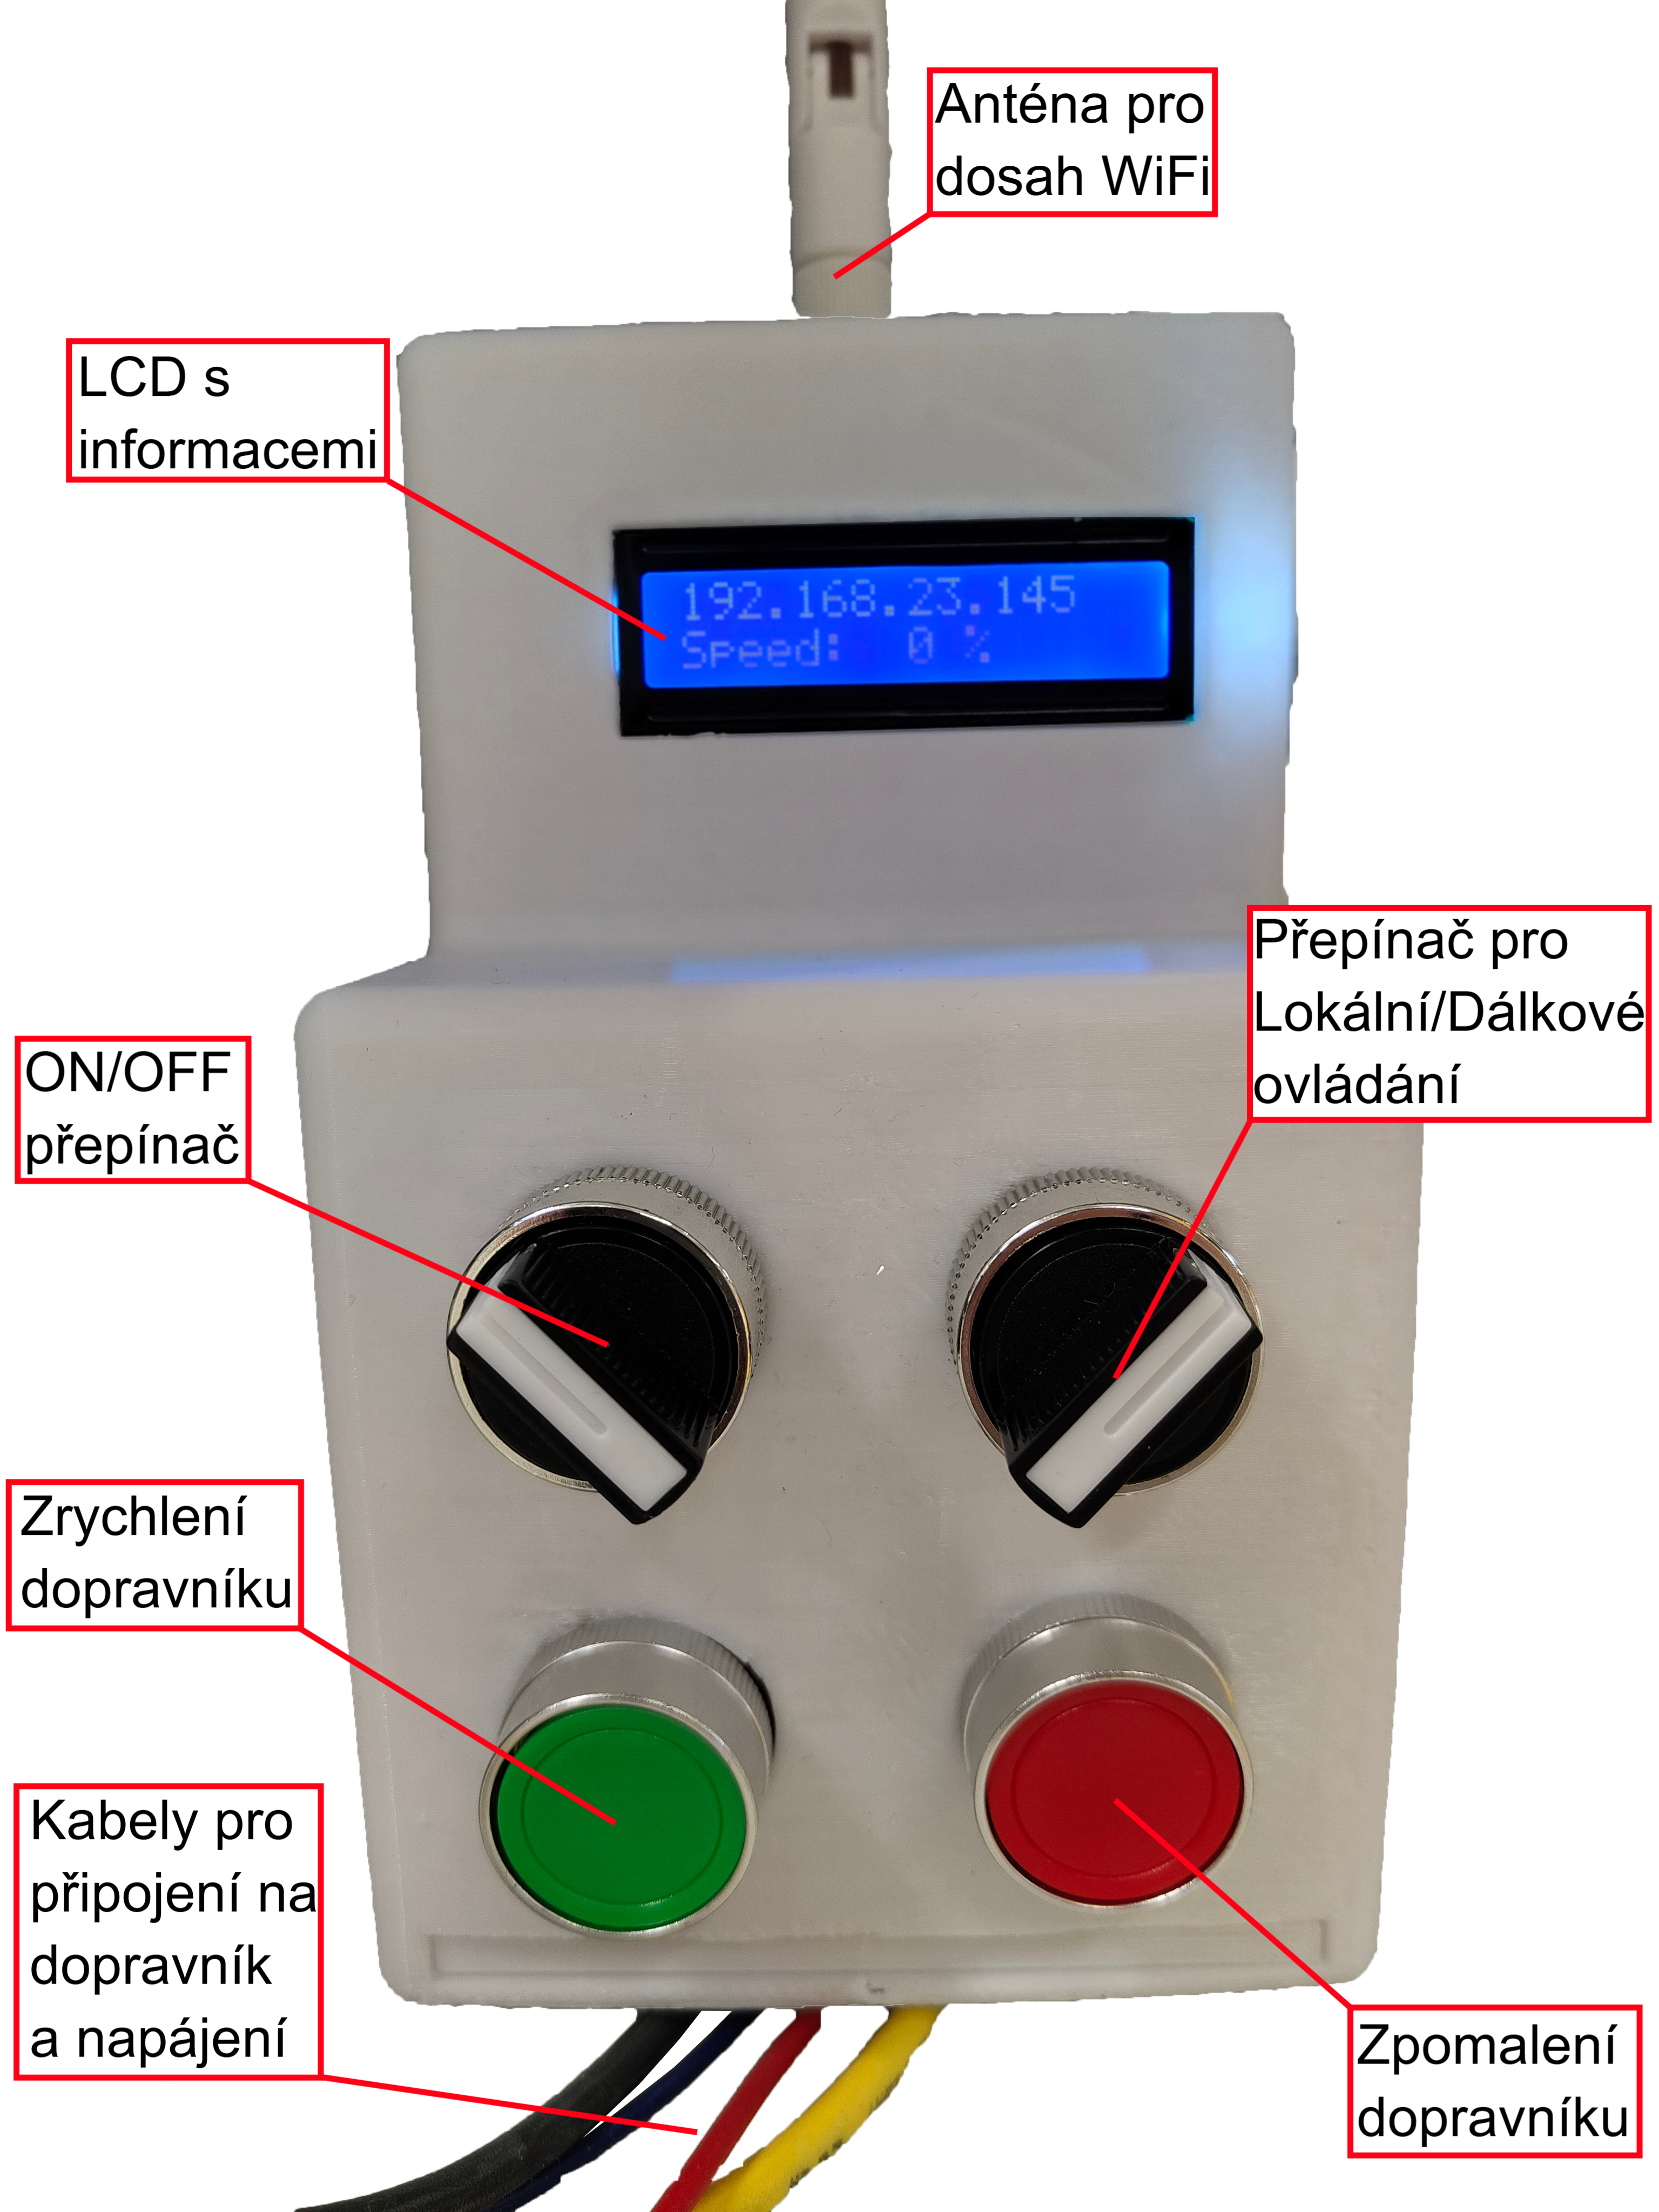
\includegraphics[width=0.5\linewidth]{images/obrazekKrabicky_annot.png}
	\caption{Popis zařízení co ovládá dopravník}
	\label{fig:PopisZarizeniCoOvladaDopravnik}
\end{figure}

Na obrázku \ref{fig:MobilniAppScreenshots} je finální vzhled mobilní aplikace. Jsou zde vidět tři hlavní strany aplikace - Nastavení, Pomoc a Ovládání. Ovládání komunikuje s vývojovou deskou tím že posílá příkazy pro ovládání dopravníku, ale také získává průběrná data o rychlosti dopravníku a typu ovládání (lokální nebo dálkové). Aplikace je dále popsaná v kapitole \ref{sec:SoftwareVMobilniAplikaci}.

\begin{figure}[hptb]
	\centering
	\begin{subfigure}[t]{0.3\textwidth}
		\includegraphics[width=\textwidth, height=290px]{images/MobilniLanding.png}
		\caption{Vstupní stránka aplikace}
		\label{fig:MobilniLanding}
	\end{subfigure}%
	\begin{subfigure}[t]{0.3\textwidth}
		\includegraphics[width=\textwidth, height=290px]{images/MobilniSetup.png}
		\caption{Část stránky nastavení}
		\label{fig:MobilniSetup}
	\end{subfigure}%
	\begin{subfigure}[t]{0.3\textwidth}
		\includegraphics[width=\textwidth, height=290px]{images/MobilniHelp.png}
		\caption{Část stránky s častými chybami}
		\label{fig:MobilniHelp}
	\end{subfigure}
	\caption{Vysílat příkazy zařízení bude mobilní aplikace připojená přes hotspot}
	\label{fig:MobilniAppScreenshots}
\end{figure}

\subsection{Požadavky na systém (0.5 strany)}\label{sec:PozadavkyNaSystem}
Pro zajištění funkčnosti a smysluplnosti návrhu je nutné si stanovit některé požadavky, které by systém měl splňovat. Tyto požadavky reflektují nejenom požadavky od společnosti Honeywell, ale i požadavky na základní spolehlivost, jednoduchost a bezpečnost ovládání dopravníků tímto způsobem.

Zde jsou požadavky, které by implementace navrženého zařízení měla splňovat:

\begin{itemize}
    \item \textbf{Lokální a dálkové ovládání}\\
    Systém bude schopný ovládat dopravníky nejenom lokálně ale i bezdrátově.
    \item \textbf{Ovládání více dopravníků zároveň}\\
    Systém by měl jednoduše zprostředkovat ovládání více dopravníků zároveň.
    \item \textbf{Ovládání z mobilního zařízení}\\
    Aby se minimalizoval počet potřebných zařízení se systém musí dát provozovat z mobilního zařízení pomocí WiFi hotspotu.
    \item \textbf{Napájení z ovládacího panelu}\\
    Systém musí být navržený tak aby jeho rozšířené funkce bylo možné napájet připojením na $24V$ výstupní port v ovládacím panelu.
    \item \textbf{Systém musí mít ovládání které je čistě analogové}\\
    Systém by měl být navržen tak, aby bylo stále možné dopravníky ovládat i pokud by něco zamezovalo napájení vývojové desky.
    \item \textbf{Uživatelská přívětivost systému}\\
    Systém by měl být uživatelsky přívětivý a jeho nastavení by mělo být jednoduše dostupné pro uživatele spolu se všemi informacemi jak s ním pracovat.
\end{itemize}

\section{Hardware}\label{sec:Hardware}
% \purpose{Jak jsem postupoval při návrhu a jak ta finální verze vypadá}

Základní stavební kámen celého systému je jeho hardware společně s deskou plošných spojů (DPS) ve které je umístěn. Celé zapojení bylo nejdříve navržené jako elektrické schéma. To bylo postupně vylepšováno, později předěláno do schématu v programu pro tvorbu DPS a nakonec bylo vytvořené rozložení komponentů přímo na desce. Pozdější verze návrhu byly provedeny v počítačovém programu na návrh desek plošných spojů jménem KiCAD. Blokové schéma funkčnosti desky lze vidět na obrázku \ref{fig:SchemaDesky}.

\begin{figure}[hptb]
	\centering
	\includegraphics[width=1\linewidth]{images/Electrical_Schematic_V2.drawio.pdf}
	\caption{Blokové schéma desky plošných spojů}
	\label{fig:SchemaDesky}
\end{figure}

Při tvorbě desky se vycházelo z požadavků na systém. Nejdřív se vycházelo z toho, že desku musí být možné napájet z ovládacího panelu, který má výstupní port na kterém je $24V$ a který je schopný dodat maximálně $8A$. Ze začátku se tedy počítalo s $24V$ napětím, pro které bylo potřeba zvolit dobrý převodník napětí co je schopný napětí přeměnit na $5V$ kterým se napájí vývojová deska. Nakonec byl zvolený převodník napětí s galvanicky oddělenou zemí aby se minimalizovala šance, že by kvůli nějaké chybě v návrhu desky byl zničený ovládací panel frekvenčního měniče.
\cite{SiemensG120DGettingStarted}

Dále se při návrhu vycházelo z myšlenky že systém musí mít i lokální i dálkové ovládání, s tím, že lokální ovládání musí být dostupné i bez napájení mikrokontroleru. Tohle bylo vyřešeno návrhem dvou přepínačů. \textit{Relé pro lokální a dálkové ovládání} je přepínač, který je normálně v poloze lokálního ovládání (aby byl splněný požadavek čistě analogového ovládání), ale pokud se na něj přidá napětí, přepne se do stavu dálkového ovládání. Následně je v desce \textit{Relé pro dálkové ovládání}, což je běžné SPST relé které sepne kontakty pokud je na něj přivedeno napětí.

Po dokončení schématu se přešlo na návrh umístění součástek na DPS. Finální návrh lze vidět v obrázku \ref{fig:PCBbothSides}. Při rozmisťování součástek po desce byl kladen důraz na několik kritérií:
\begin{itemize}
	\item Aby měla deska co nejmenší rozměry a měla jen dvě vrstvy
	\item Aby byly všechny součástky na jedné straně desky (jednodušší pájení komponentů na desku)
	\item Aby byly trasy co nejkratší
	\item Aby měla deska co nejméně vertikálních cest (pro zmenšení efektů parazitní kapacity a parazitní indukčnosti)
	\item Aby byly filtrační kondenzátory co nejblíž filtrovaných napájecích vstupů
\end{itemize}

\begin{figure}[hptb]
	\centering
	\begin{subfigure}[t]{0.48\textwidth}
		\includegraphics[width=\textwidth]{images/PCBfront.png}
		\caption{Přední strana DPS}
		\label{fig:PCBfront}
	\end{subfigure}%
	\hfill
	\begin{subfigure}[t]{0.48\textwidth}
		\includegraphics[width=\textwidth]{images/PCBback.png}
		\caption{Zadní strana DPS}
		\label{fig:PCBback}
	\end{subfigure}
	\caption{Návrh desky plošných spojů v KiCAD}
	\label{fig:PCBbothSides}
\end{figure}

\subsection{Ovládání relé}
Jedna z věcí které bylo potřeba vyřešit při návrhu schématu elektrického obvodu je taková, že bylo cílem ovládat relé pomocí výstupních pinů vývojové desky. Pro spuštění relé je ovšem potřeba brát na paměť, že vyžaduje nejenom napětí $5V$ na ovládacím pinu, ale také vyžaduje proud do cívky $133mA$. Vývojová deska je schopná svými výstupními piny poskytnout napětí $5V$, ale její výstupní proud je pouze $10mA$. Tento problém je možné vyřešit pomocí tranzistorů.

Nejjednodušší řešení pro navrženou desku je řešení s N kanálovým NPN tranzistorem MOSFET, jelikož v případě MOSFET tranzistorů obecně stačí aby signál byl napěťový (nemusíme tedy řešit malý proud vycházející z vývojové desky). Nejdřív se relé zapojí tak, aby cívka měla na jedné straně $5V$ napětí a na druhé straně zem. Následně se MOSFET tranzistor dá mezi zem a cívku a na bázi tranzistoru se přivede signál z mikrokontroleru. V tomto zapojení bude skrz relé téct nominální proud, pokud je výstup vývojové desky vysoký, anebo bude obvod rozpojený pokud bude výstup z vývojové desky na nízké hodnotě napětí.

Dále je potřeba ještě paralelně s relé zapojit diodu kvůli ochraně tranzistoru od vybíjecího proudu co cívka generuje po rozpojení obvodu. Tato dioda musí mít v závěrném směru hodnotu napětí vyšší než je $5V$ napětí zdroje a musí se zapojit tak, aby byla otevřená když se otočí polarita napětí na cívce v relé. Pro tuto desku byla zvolena Schottkyho dioda kvůli její rychlosti přepínání a kvůli malému napětí které se na diodě v otevřeném stavu nachází.

Na obrázku \ref{fig:OvladaniRele} je schéma zapojení tohoto způsobu ovládání relé pomocí vývojové desky.

\begin{figure}[hptb]
	\centering
	\includegraphics[width=0.6\linewidth]{images/OvladaniRele.drawio.pdf}
	\caption{Elektrické schéma ovládání relé}
	\label{fig:OvladaniRele}
\end{figure}

\subsection{LCD display s I2C převodníkem}
Aby bylo možné celý systém ovládat přes ESP8266 WebServer, je potřebné nějakým způsobem komunikovat s uživatelem IP adresu, kterou má vývojová deska připojená na hotspot mobilního zařízení. Tohle by bylo možné udělat například skrz nastavení multicast DNS na specifickou adresu a tu potom fyzicky napsat na schránku desky. Toto řešení by sice umožnilo přístup k WebServeru, ale neposkytovalo by to další funkce jako systém může mít se zabudovaným LCD displejem do desky plošných spojů.

Použití LCD displeje v systému může uživateli dodávat tyto informace:
\begin{itemize}
	\item Stav připojení mikrokontroleru k hotspotu (před navázáním spojení systém nemůže reagovat na požadavky přes WebServer).
	\item Název (SSID) a heslo hotspotu, které mikrokontroler očekává.
	\item Aktuální rychlost dopravníku.
	\item IP adresu pro přístup k WebServeru.
\end{itemize}

Na základě uvedených důvodů a požadavků na rozsah poskytovaných informací byl pro komunikaci s uživatelem zvolen LCD displej.

Konkrétně byl použit 16x2 znakový LCD displej (obrázek \ref{fig:LcdDisplej}) zakoupený v internetovém obchodě LaskaKit \cite{laskakit_16x2_lcd}. Tento model je vybaven připájeným I2C převodníkem, což zjednodušuje jeho připojení na pouhé čtyři vodiče: dva pro I2C sběrnici (Serial Data (SDA) a Serial Clock (SCL)), jeden pro napájení $5V$ a jeden zemnící vodič (GND). Výhodou zvoleného displeje je také dostupnost knihovny pro Arduino framework, což usnadňuje jeho softwarovou implementaci ve firmwaru mikrokontroleru.
\cite{laskakit_16x2_lcd}

\begin{figure}[hptb]
	\centering
	\begin{subfigure}{0.48\textwidth}
		\includegraphics[width=1\textwidth]{images/predni_LCD_s_I2C.jpg}
		\caption{Přední strana}
		\label{fig:PredniLCDDisplej}
	\end{subfigure}
	\hfill
	\begin{subfigure}{0.48\textwidth}
		\includegraphics[width=1\textwidth]{images/zadni_LCD_s_I2C.jpg}
		\caption{Zadní strana}
		\label{fig:ZadniLCDDisplej}
	\end{subfigure}
	\caption{LCD displej s I2C převodníkem \cite{laskakit_16x2_lcd}}
	\label{fig:LcdDisplej}
\end{figure}

Vzhledem k citlivosti komunikace po I2C sběrnici na elektromagnetické rušení a přeslechy byly při návrhu desky plošných spojů dodrženy zásady pro minimalizaci smyčkové plochy mezi signálovými cestami SDA a SCL. Tento postup snižuje indukované napětí a přispívá ke spolehlivosti přenosu dat na sběrnici.
\cite{CurrentLoopsBlog}

Pro jednoduchost výměny LCD displeje bylo také zvoleno, že nebude přímo připájený v desce, ale podobně jako vývojová deska bude připojený skrz kolíkové lišty. Tohle zjednodušuje výměnu nebo upravení parametrů LCD displeje jako je jas zobrazených písmen.

% Tyhle veci nebudu popisovat, protože stačilo napsat, že mám ten převodník napětí co mění z 24V na 5V a je galvanicky oddělený. Není potřeba víc to rozepisovat
%\subsection{Převodník napětí 24V-5V (1 strana)}
%\purpose{Tady vysvětlím že používám tenhle převodník napětí, nějaký jeho specifikace, podle kterých jsem si ho zvolil. }
%\purpose{Vysvětlit jaký specifický hardware součásti jsem do desky dal a proč jsem se rozhodl je tam dát.}
%
%\subsection{LC Filtr napájecího napětí (1 strana)}
%\purpose{Sem napsat jak jsem navrhoval LC filtr za napájecím napětí, proč jsem se rozhodl použít LC filtr a třeba by se sem mohl hodit nějakej grafík přenosové funkce kdybych se nudil. Zvolil jsem si cutoff aby byl alespoň 1/10 hodnoty na které měnič dělá šum a díky tomu by měla hodnota tohoto šumu být o 20dB menší.}
%\purpose{Vysvětlit jaký specifický hardware součásti jsem do desky dal a proč jsem se rozhodl je tam dát.}

\section{Firmware ve vývojové desce}
% \purpose{Tady bych rád trochu vysvětlil jak funguje software ve vývojové desce.}

Jak bylo již napsáno v kapitole \ref{sec:ArduinoFrameworkForESP8266} tento projekt byl programovaný v prostředí PlatformIO. Tohle programovací prostředí má tu výhodu v tom, že pro programování vývojových desek si stačí vybrat typ vývojové desky, kterou programuji a dané prostředí se nakonfiguruje tak, aby to bylo možné (V případě WEMOS D1 Mini Pro byl implementován Arduino framework pro ESP8266). Z tohoto prostředí tedy lze programovat jakékoliv vývojové desky a programovat je jakýmkoliv jazykem mezi které patří například Arduino jazyk anebo MicroPython. Pro firmware v tomto projektu byl zvolený Arduino framework a tak je programovací jazyk Arduino verze C++.
\cite{PlatformIOWeb}

Honeywell je anglicky mluvící firma a tak je celý firmware i software v mobilní aplikaci programovaný anglicky.

V C++ programovacím jazyku se běžně objevují dva hlavní typy souborů. Jsou to hlavičkové soubory (s koncovkou \textit{.h}) a zdrojové soubory (s koncovkou \textit{.cpp}). Zatímco hlavičkové soubory obsahují deklarace, jako jsou prototypy funkcí nebo definice globálních proměnných, zdrojové soubory obsahují implementace a kód který je následně kompilován a prováděn na mikrokontroleru. V tomto projektu jsou dva hlavičkové a dva zdrojové soubory.

Jeden hlavičkový soubor obsahuje definice alternativních názvů pro výstupních a vstupních piny GPIO vývojové desky aby bylo jednodušší se orientovat v kódu. Dále je zde soubor \textbf{main.cpp}, který kompilátor přirozeně vyhledává aby v něm nastavil začátek provádění kódu. Nakonec je zde zdrojový a hlavičkový soubor s názvem \textbf{ConveyorController} který definuje třídu a zdrojový kód objektu který celý systém řídí.

\subsection{Třída a objekt ConveyorController}\label{sec:ConveyorController}
% \purpose{V kódu všechno ovládám pomocí tohoto objektu, který obsahuje hodně public a private funkcí. Tady bych chtěl vysvětlit z jakýho důvodu jsem se rozhodl vývojovou desku ovládat tímto způsobem a dále vysvětlit co jednotlivé důležité metody a proměnné dělají.}

C++ je objektově orientovaný program a tak má rozsáhlé funkce pro definici vlastních tříd. Kvůli tomu je důležité rozlišovat mezi pojmy třída a objekt. Třída v C++ slouží jako abstraktní definice pro vytvoření nového uživatelsky definovaného datového typu. Objekt je na druhou stranu konkrétní instance třídy a tak má alokované místo v RAM paměti a je sledovaný jeho unikátní stav během provádění kódu.
\cite{CppObjectAndClassArticle}

Hlavní výhodou proč byl v práci použitý objektově orientovaný přístup je kvůli zavedení takzvané \textbf{enkapsulace} uvnitř kódu. Jinými slovy, umožňuje to separaci řídící logiky dopravníku od zbytku aplikačního kódu. Během implementace firmwaru vyvstala potřeba, aby určité proměnné, jako například proměnná \textit{conveyorSpeed} reprezentující aproximaci rychlosti dopravníku či proměnná \textit{remoteLocalState} indikující stav řízení (vzdálené/lokální), byly přístupné napříč několika funkcemi. Běžně by bylo možné tyto proměnné řešit pomocí globálních proměnných, ale to je v komplexnějších firmwarech považováno za rizikové.
\cite{EnkapsulaceVCppArikl}

V takovém případě se pro bezpečnější provádění kódu může přejít k využívání objektů. Samotný objekt je sice definovaný globálně, ale uvnitř má tři definice přístupu: \textbf{veřejný, privátní a chráněný}. Tímto způsobem se může pro jakékoliv proměnné uvnitř objektu určit, v jakých částech kódu budou dostupné, s tím, že pokud je proměnná definovaná jako veřejná, dá se získat i mimo daný objekt a na druhou stranu pokud je proměnná privátní, je možné ji získat pouze uvnitř metod objektu. Metoda je taková funkce, kterou je možné uvnitř objektu se stejnými přístupy definovat a je to kus kódu co bude provedený pokud bude metoda zavolaná. Metody které jsou veřejné je tedy možné spouštět ze skriptu \textit{main.cpp} ve kterém existuje globální instance objektu, ale privátní metody už není možné z hlavního skriptu spouštět.

Kvůli této funkcionalitě bylo od začátku rozhodnuto, že bude kód programovaný tímto způsobem. Většina kódu bude obsažena v conveyorController objektu a v hlavním zdrojovém kódu budou pouze volány veřejné metody této globální instance třídy ConveyorController.

Aby bylo možné představit jaké funkce jsou v ConveyorController třídě obsaženy, zde je její definice v hlavičkovém souboru \textit{ConveyorController.h}:

\input{codes/ConveyorControllerHeader}

Z této definice lze vidět, že pro přehlednost je celkový kód rozdělený do různých metod tak, aby měla každá metoda svůj účel. Tyto metody jsou seřazené podle pořadí provedení až do funkce startTicker, po které se už funkce provádějí periodicky. Účely které zajišťují metody jsou:

\begin{itemize}
	\item \textbf{initIO} - Nastavuje piny vývojové desky na vstupy a výstupy pomocí PinMode příkazu a dále inicializuje výstupní piny na nízkou hodnotu.
	\item \textbf{initLCD} - Inicializuje používání LCD displeje.
	\item \textbf{initWeb} - Začne hledání webové sítě, která by odpovídala parametrům nastaveného jména (SSID) a hesla. Také informuje o hledání sítě na LCD displeji a přes serial komunikaci, kterou se hodí mít při debugování firmware.
	\item \textbf{assignRoutes} - Přiřadí WebServeru odpovědi na jednotlivé adresy. Tyto odpovědi obsahují nejdříve nastavení \textit{<head>} části odpověďi (dále vysvětlené v kapitole \ref{sec:KonvertovaniWeboveAplikaceDoMobilni}), poté provádění C++ kódu a nakonec odesílání odpovědí na požadavky.
	\item \textbf{startWebServer} - Spustí WebServer, který bude nyní přijímat požadavky.
	\item \textbf{startTicker} - Nastaví Ticker (časovač) pro periodické spouštění hlavní funkce \textbf{updateState} a funkce pro aktualizaci LCD.
	\item \textbf{handleClient} - Sleduje webové požadavky.
	\item \textbf{updateLCD} - Aktualizuje na LCD displeji hodnotu IP adresy a hodnotu rychlosti dopravníku.
	\item \textbf{updateState} - Tato funkce řídí relé na desce plošných spojů a tak i ovládá celý dopravník. Chová se dle stavového diagramu, který je popsaný v kapitole \ref{sec:UpdateStateStavovyDiagram}.
\end{itemize}

Hlavičkový soubor dále obsahuje i několik prototypů privátních metod které urychlují psaní kódu při opakovaných úkonech a proměnných které jsou používáné uvnitř metod (všechny proměnné používané uvnitř třídy jsou privátní). Specifické privátní metody které je potřeba poukázat jsou metody \textbf{mainRoute} a \textbf{unknownRouteReponse}. Tyhle metody zahrnují vytváření HTML řetězce kterým se odpovídá na webové požadavky, co přichází na WebServer. Je to podobný způsob jak odpovídat na webové požadavky jako byl v ukázce kódu \ref{lst:NastaveniWebServeru}.

\subsection{Stavový diagram logiky systému (5 stran)}\label{sec:UpdateStateStavovyDiagram}
%\purpose{Vysvětlit jak funguje funkce v kódu která se chová na základě stavového diagramu}

Aby bylo možné řídit dopravník pomocí ConveyorController objektu, je potřebné implementovat v kódu logiku, která sleduje stav ovládání dopravníku a podle stavu ovládání bude spínat tranzistory co spouští relé v desce plošných spojů. Do téhle funkcionality se navíc dalo přidat i některé další funkce jako je aproximace rychlosti dopravníku blíže popsaná v kapitole \ref{sec:AproximaceRychlostiDopravniku}. Tato veřejná metoda objektu ConveyorController se jmenuje updateState a je pomocí knihovny Ticker prováděna každých 300 milisekund.

V tomhle systému je na tuto část kódu nahlíženo jako na stavový diagram Harelova typu. Pro přehlednost je zde stavový diagram rozdělený do tří různých částí (byl ale navrhován jako jeden celek):
\begin{itemize}
	\item \textbf{Začátek stavového diagramu} - kde se rozhoduje hlavně jestli je dopravník řízený lokálně nebo dálkově.
	\item \textbf{Dálkové ovládání dopravníku}
	\item \textbf{Lokální ovládání dopravníku}
\end{itemize}

\begin{figure}[H]
	\centering
	\includegraphics[width=1\linewidth]{images/StateFlow_Firmwaru_top.drawio.pdf}
	\caption{Začátek stavového diagramu}
	\label{fig:StateFlow_Firmwaru_top}
\end{figure}

Zde je vstup do stavového diagramu funkce updateState. Na začátku se přečte hodnota vstupního pinu vývojové desky ke kterému je připojený přepínač pro lokální nebo dálkové ovládání. Na základě této hodnoty se určí, jestli je systém ve stavu lokálního nebo dálkového ovládání. Podle této hodnoty se stavový diagram větví do diagramů pro lokální nebo dálkové ovládání.

\begin{figure}[H]
	\centering
	\includegraphics[width=1\linewidth]{images/StateFlow_Firmwaru_left.drawio.pdf}
	\caption{Strana stavového diagramu s lokálního ovládáním}
	\label{fig:StateFlow_Firmwaru_left}
\end{figure}

Ve stavu s lokálním ovládáním se nastaví výstupní pin vývojové desky ovládající tranzistor, který vypne relé, které přepíná mezi lokálním a dálkovým ovládáním. Následně se rovněž nastaví tranzistor ovládající dálkové ovládání, jelikož není potřeba toto relé mít zapnuté, když je tato větev obvodu deaktivována. Nakonec se nastaví proměnné dálkového ovládání na FALSE, aby byly vynulovány nastavené příkazy z WebServeru. Na konci provedení těchto bloků kódu se přečtou stavy tlačítek a přepínačů umístěných fyzicky na desce a na základě těchto stavů se pokračuje v provádění kódu.

V tomto stavu působí mikrokontroler spíše jako pouhý pozorovatel stavu tlačítek, než aby přímo spínal nějaké z relé. V blokovém schématu systému na obrázku \ref{fig:SchemaDesky} lze vidět, že tomu tak je protože je relé pro přepínání lokálního nebo dálkového ovládání připojené přímo k tlačítku, které bez žádného digitálního zpracování spíná nebo rozepíná 24V linku napětí pro ovládací panel. Toto vychází z požadavku na systém \textbf{Systém musí mít ovládání které je čistě analogové}.

Ze začátku se může pokračovat do větve \textbf{Dopravník je lokálně vypnutý}, a to v případě, že je hodnota přepínače, který lokálně ovládá stav ON/OFF, vyhodnocena LOW. V tomto stavu se pouze odečte hodnota rychlosti dopravníku, pokud je rychlost vyšší než 0 \footnote{rychlost dopravníku sledovaná v proměnné conveyorSpeed je pouze aproximace, která se zobrazuje v mobilní aplikaci a na LCD displeji. Není to vstup do ovládacího panelu.}.

Alternativně je možné pokračovat do větve \textbf{Dopravník je lokálně zapnutý}, pokud je hodnota přepínače ON/OFF vyhodnocena jako HIGH. V tomto případě se sleduje, jakým způsobem je dopravník ovládán, a na základě toho se přičte nebo odečte hodnota rychlosti dopravníku.

\begin{figure}[H]
	\centering
	\includegraphics[width=1\linewidth]{images/StateFlow_Firmwaru_right.drawio.pdf}
	\caption{Strana stavového diagramu s dálkovým ovládáním}
	\label{fig:StateFlow_Firmwaru_right}
\end{figure}

Ve stavu s dálkovým ovládáním se nastaví výstupní pin, který ovládá relé pro dálkové nebo lokální ovládání, na úroveň HIGH. V rámci tohoto stavu už není nic dalšího provedeno, jelikož se proměnné, na základě kterých se ve stavovém diagramu pokračuje, nastaví při zpracování GET požadavků, které přicházejí na WebServer.

WebServer tedy nastavuje proměnné, na základě kterých se v tomto stavovém diagramu pokračuje v provádění kódu. Tyto proměnné jsou inicializovány na hodnotu FALSE, a proto se po přepnutí do režimu dálkového ovládání dopravník vypne. Během provádění stavového diagramu dálkového ovládání nejsou tyto hodnoty vynulovány, a je proto nutné přes WebServer nastavit proměnné jak na hodnotu TRUE, tak na hodnotu FALSE.

Pokud přes WebServer bude proměnná ON/OFF nastavena na hodnotu FALSE, poté se vypne relé, které ovládá dálkové ovládání, a sníží se hodnota rychlosti dopravníku až na 0.

Pokud se přes WebServer proměnná ON/OFF nastaví na hodnotu TRUE, sepne se tranzistor, který přivede proud do relé pro dálkové ovládání. Podobně se spustí relé, které zrychluje nebo zpomaluje dopravník přes ovládací panel, pokud jsou jejich specifické proměnné nastavené na hodnotu TRUE. Také zde se zvyšuje nebo snižuje hodnota aproximace rychlosti.

%%%%%%%%%%%%%%%%%%%%%%%%%%%%%%%%%%%%%%%%%%%%%%%%%%%%%%%%%%%%%%%%%%%%%%%%%%%%%%%%%%%%%%%%
\oldtext
%%%%%%%%%%%%%%%%%%%%%%%%%%%%%%%%%%%%%%%%%%%%%%%%%%%%%%%%%%%%%%%%%%%%%%%%%%%%%%%%%%%%%%%%

\subsubsection{Jak aplikace aproximuje rychlost dopravníku}\label{sec:AproximaceRychlostiDopravniku}
\purpose{Vysvětlit jak se pomocí Tickeru aproximuje rychlost dopravníku}

Aplikace aproximuje rychlost dopravníku tak, že předpokládá že dopravník ovládaný frekvenčním měničem zrychluje lineárně - což je běžná praxe pro frekvenční měniče kvůli důvodům popsané v kapitole \ref{sec:JakFungujiFrekvencniMenice} a je to něco co jsem si potvrdil když jsem na dopravníku zkoušel funkčnost zařízení. Dává to smysl, protože tohle zrychlování je čistě softwarová záležitost frekvenčního měniče a tak není důvod proč by nebylo lineární. Během testování jsem zjistil, že frekvenční měnič má ramp up time sice nastavený na 10 sekund, ale za těch 10 sekund dosáhne $500 ot/min$. Pokud bych chtěl tedy zrychlit dopravník z nulové rychlosti na maximální rychlost 1500 otáček za minutu, musím počkat čas 3x větší než je jeden ramp up time. Dopravník stejnou rychlostí i zabrzďuje.

Samotná aproximace rychlosti je implementována ve funkci updateState, která je blíže vysvětlená ve kapitole \ref{sec:UpdateStateStavovyDiagram}. Aproximace je provedena hned po nastavení výstupních pinů v rámci updateState vývojové desky tím, že se přičte nebo odečte hodnota proměnné conveyorSpeed. Proměnná conveyorSpeed je nastavená jako celé číslo a reprezentuje procento rychlosti z maximální rychlosti. Jelikož se funkce updateState volá každých 0.3 sekundy a během každého zavolání se buďto zvýší conveyorSpeed pokud se zrychluje, nebo sníží conveyorSpeed pokud se zpomaluje, dosáhne maximální hodnoty 100 za 30 sekund, což je čas potřebný pro dosáhnutí maximální rychlosti dopravníku.

Funkce updateState se volá zaokrouhleně 3x za sekundu a takové rozlišení by mělo stačit pro to aby aproximace nenabývala hodnot drasticky mimo z důvodu např. rozpojení tlačítka těsně předtím než se provede updateState.

Tahle funkcionalita dává inženýrům co kontrolují dopravníky důležité informace o rychlosti i bez toho aby k dopravníku museli mít připojené zařízení jako BOP-2 z kapitoly \ref{sec:NastaveniOvladacihoPanelu} vysvětlující nastavení ovládacího panelu dopravníku.

\section{Software v mobilní aplikaci ($\Sigma$ = 5 stran)}\label{sec:SoftwareVMobilniAplikaci}
\purpose{V téhle sekci popíšu jak přesně funguje mobilní aplikace kterou jsem vytvořil a poznatky s tím spojené.}

Jak už jsem nastínil v \ref{sec:PopisFunkceSystemu} tak hlavní motivace proč navrhuji mobilní aplikaci je kvůli tomu aby nebylo potřeba mít extra zařízení pro ovládání dopravníků. Díky mobilní aplikaci můžu vytvořit zařízení které umožní dopravníky ovládat na vzdálenost 10-100 metrů (vzdálenost WiFi protokolu - \source{zdroj needed}) a stačí mi navrhnovat jenom zařízení které se připojí na dopravník a už nemusím navrhovat zařízení, které signály vysílá. To zmenšuje počet krabiček co musí zaměstnanci software tahat s sebou.

Výhodou mobilní aplikace je taková, že můžu na jedno místo dát všechny návody - můžu tak mít setup i všechno ovládání v rámci jedné aplikace což je rozhodně lepší než to mít v pdf dokumentu někde mimo. Pomáhá mi to tak na jeden z požadavků kdy jsem chtěl aby byl systém jednoduchý a intuitivní na používání.

\subsection{Architektura aplikace}
\purpose{Vysvětlit jakým způsobem jsem navrhoval architekturu aplikace a proč. Architektura = statická frontendová webová aplikace převedená do mobilní podoby pomocí WebView. Výhody jsou jednoduchost implementace GET requestů ve webové aplikaci. Zde taky přestavit React a Capacitor.}

Ta aplikace samotná je čistě frontendová (statická) webová aplikace postavná na Vite verzi Reactu. Capacitor tuhle aplikaci převádí do mobilní aplikace a kvůli tomu potřebuju používat některý balíčky spojený s capacitorem aby mi to umožnilo posílat webové požadavky na IP adresy nodeMCU serverů.

\textbf{Webová aplikace má tři URL adresy:}
\begin{itemize}
    \item Vstupní stránka - Tato stránka obsahuje hlavní část aplikace která umožňuje ovládání dopravníků.
    \item Setup - Tato stránka obsahuje návod jak dopravník nastavit aby s tímto zařízením správně fungoval.
    \item Help - Tato stránka obsahuje časté chyby které můžou nastat při používání zařízení a při nastavování dopravníků a snaží se poskytnout rady aby pomohla s vyřešením problémů.
\end{itemize}
Tyto URL adresy jsou převedené i do adres dostupných na mobilní aplikaci. Navigaci na tyto adresy zajišťuje header s navbarem jelikož v android WebView nelze zadávat URL adresy a tak musí navigace probíhat přes tlačítka na webu.

\purpose{Co je to React a proč se hodí na návrh této webové aplikace. Co je to HTML, CSS a JS. Co je to reaktivnost komponentů. Jak se react využívá. Možná sem přidat co je to tailwind a Lucide for React.}

React je web developmentovej framework a hodí se na návrh, protože přes node package manager už existují frameworky, který mi umožní webový aplikace portovat do mobilní aplikace - tenhle framework se jmenuje capacitor. Capacitor používá WebView (pro Android) nebo WKWebView (pro iOS) a díky tomu umožňuje zobrazit si webové aplikace na zařízení.\cite{CapacitorDocumentationFAQ}

Webovou aplikaci navrhuji, protože to, co chci aby dělala je aby jenom posílala GET požadavků na IP adresu mikrokontrolleru kterou hostuje NodeMCU, což je hodně jednoduchá věc na implementaci ve webové aplikaci.

\source{React může mít zase jako zdroj nějakou odbornou literaturu zaměřenou na react (pokud něco takového najdu) anebo online dokumentaci.}

\subsection{Použité knihovny a technologie v aplikaci (0.5 strany)}
\purpose{Vysvětlit co za frameworky (knihovny) jsem při developování aplikace použil aby to fungovalo co nejlépe}

\subsubsection{HTML, CSS a JS}

\subsubsection{TypeScript}

\subsubsection{Tailwind}

\subsubsection{DaisyUI}

\subsubsection{Lucide for React}

V rámci programování jsem používal několik rozšíření, které web developerům pomáhají v designu aplikací. Tím je \textbf{Tailwind}, což je rozšíření které umožňuje stylizovat kód webové aplikace pomocí vlastnosti className, kterou mají veškeré HTML prvky a tím není potřeba mít samostatné soubory v CSS (jazyk který webům dává jejich design). Na Tailwind navazuje rozšíření \textbf{DaisyUI}, které zjednodušuje celkový design aplikace tím, že mi umožňuje si nadefinovat barvy motivu aplikace v různých proměnných, díky čemuž je možné motiv měnit skrz změnu jedné promenné nastaveného motivu. Také umožňuje mít vlastní styl aplikace pokud má mobilní zařízení temný režim nebo světlý režim. S designem aplikace ještě pomáhalo rozšíření \textbf{Lucide pro React}, které obsahuje velké množství ikon pro různé prvky uživatelského rozhraní, jako je třeba ve tlačítkách ON/OFF, Add Conveyor, zrychlení, atd.

Aplikace ještě používá TypeScript, což je nadstavba JavaScriptu, která umožňuje definovat typy proměnných, což zvyšuje bezpečnost programu a zlepšuje zážitek z programování, vzhledem k tomu, že programátory upozorňuje na chyby v kódu, na které by JavaScript běžně neupozornil.

\subsection{Princip komunikace s NodeMCU servery}
\purpose{Co je to GET požadavek a jak se dá implementovat v JavaScriptu.}

\purpose{Jak se GET požadavek mění když používám capacitor}

\subsubsection{Co je to GET požadavek }
\purpose{Vysvětlit obecně jak fungují GET požadavky z web developmentu}

Aplikace bude ovládat nodeMCU servery přes posílání webových GET požadavků. GET požadavek je typicky například když do prohlížeče na PC zadám do URL adresy jakýkoliv název webu - tak to provádím GET požadavek na server, který je na IP adrese hostován. V tomhle případě jsou servery moje nodeMCU servery a místo PC zadávám požadavky přes webovou aplikaci.

V rámci nodeMCU se nastavují adresy na kterých server nějakým způsobem odpovídá. Během tohoto nastavení můžu nejenom určit jaká stránka se ukáže po zadání požadavku na získání informací z webové adresy, ale můžu tím spouštět i jakýkoliv jiný kód.

Typický test této funkce je pomocí GET požadavku na IP adresu rozsvítit LED diodu, která přes breadboard zapojená do výstupního pinu vývojové desky WEMOS D1 mini pro. Pokud je deska připojená ke stejné WiFi síti jako můj počítač, můžu na počítači zadat například adresu 192.168.0.144/ledON. NodeMCU server na tuto adresu odpoví tím, že změní stav LED diody v desce a až poté pošle zpátky HTML kód, který se mi zobrazí v prohlížeči. Takto je možné provádět jakýkoliv kód, který je nastaven aby se prováděl v rámci GET požadavků na jakoukoliv adresu.

V reactu se běžně GET požadavky provádí pomocí asynchronní funkce fetch. Asynchronní funkce jsou speciální funkce, během kterých můžeme používat speciální slovo "await". Tohle slovo způsobí, že Javascript počká než se daný příkaz dokončí a až poté bude pokračovat v provádění funkce. Tohle zamezuje vznik chyb v kódu, které můžou vznikat pokud se snažím dělat operace s proměnnými, které jsou zatím prázdné (jelikož ty data ještě například neposlal server).

V běžné react aplikaci by bylo možné posílat GET požadavky na nodeMCU server tímto způsobem:

\begin{lstlisting}[language=JavaScript, caption={Základní způsob posílání GET požadavků v JavaScriptu}, label={lst:JavaScriptFetchFunkce}]
async function getData() {
  const url = "https://example.org/products.json";
  try {
    const response = await fetch(url);
    if (!response.ok) {
      throw new Error(`Response status: ${response.status}`);
    }

    const json = await response.json();
    console.log(json);
  } catch (error) {
    console.error(error.message);
  }
}
\end{lstlisting}

\source{MDN web docs}

\subsubsection{Implementování GET requestů do aplikace}
\purpose{Vysvětlit proč normální GET requesty nefungují (Omezení z WebView) a jak je tedy implementovat. Taky zmínit že jsou implementované ve funkci sendCommand.}

GET požadavky není kvůli capacitoru možné posílat běžným způsbem, protože v android aplikaci nefunguje fetch funkce tak, jak se od ní očekává. Je ale možné použít balíček vytvořený komunitou capacitoru který se jmenuje CapacitorHttp (což bylo nedávno přidané do základního capacitor balíčku). je to balíček, který zjednodušuje posílání GET požadavků na servery v rámci Capacitor aplikací tím, že má metodu GET, která funguje jako běžný fetch požadavek typu GET, ale je upravený aby fungoval ve WebView mobilním prostředí.

Tímto způsobem se v aplikaci posílají GET požadavky:
\begin{lstlisting}[language=JavaScript, caption={Funkce sendCommand dostupná uvnitř vstupní stránky aplikace}, label={lst:SendCommandFunkce}]
    // pred zacatkem komponentu:
    import { CapacitorHttp } from "@capacitor/core";
    import { HttpOptions } from "@capacitor/core/types/core-plugins";

    // uvnitr komponentu se strankou aplikace:

      // Send a command to a specific conveyor and update its status
  const sendCommand = async (ip: string, command: string) => {
    try {
      const options: HttpOptions = {
        url: `http://${ip}/${command}`,
      };

      const response: any = await fetchWithTimeout(
        CapacitorHttp.get(options),
        3000 // Fail fast if conveyor is unresponsive
      );

      setErrorMessage(null);
      console.log(response);
      try {
        const responseData = await response.json();
        console.log("Response data:", responseData);
      } catch (error: any) {}
    } catch (error: any) {
      console.error("Command failed:", error);
      setErrorMessage(`Command failed for ${ip}: ${error.message}`);

      // Immediately mark the conveyor as offline when a command fails
      setConveyors((prevConveyors) =>
        prevConveyors.map((conv) =>
          conv.ip === ip ? { ...conv, isOnline: false } : conv
        )
      );
    }
\end{lstlisting}
Nejdřív je nutné si importovat HttpOptions a CapacitorHttp z capacitoru. Následně pokračuje definice komponentu, který obsahuje celou vstupní stránku aplikace. Uvnitř stránky aplikace je definovná funkce sendCommand.

Funkce sendCommand má jako vstupy IP adresu a adresu na kterou bude posílat GET požadavek. Princip je takový, že se do HttpOptions nastaví jako URL celá IP adresa i s adresou požadavku a to se pomocí CapacitorHttp.get funkce pokusí získat. Pokud byl požadavek úspěšně doručen, aplikace se bude pokoušet přeložit odpověď přes json syntaxi, ale to se často pokazí, protože aplikace v rámci některých odpověďí odpovídá i HTML kódem aby bylo možné ji ovládat i přes webový prohlížeč. Pokud se tedy přeložit odpověď nepovede, není to žádný problém a proto je v pořádku mít řádek s přeložením ze json souboru ve try catch bloku, který jakýkoliv error potlačí.

Pokud funkce nezíská odpověď do 3 sekund, kód aplikace pomocí fetchWithTimeout (moje vlastní funkce definovaná jinde v kódu) vyšle error, který do konsole vypíše, že požadavek z nějakého důvodu nebyl doručen a zároveň zobrazí i error v uživatelském rozhraní aplikace. Tohle je obzvlášť důležitá funkce, protože se uživateli v aplikaci ukáže error pokud v rámci času 3 sekund nodeMCU server neodpoví na požadavek - informuje to tedy o tom, že uživatel buďto zadal špatnou adresu, anebo odešel z dosahu ve kterém je nodeMCU server schopný se připojit na WiFi hotspot jeho mobilního zařízení. Tato implementace také vypíná možnost mačkat tlačítka, které ovládají dopravník, vzhledem k tomu, že by tlačítko vůbec nic nedělaly.

\subsection{Funkčnost aplikace (hodně stran)}
\purpose{Tady už vůbec neřešit jak ta aplikace vypadá, ale zaměřit se na to co ta aplikace dokáže a jak to dělá. Struktura hlavní stránky, správa seznamu dopravníků, ovládání dopravníků je zahrnuto v sendCommand, získávání a zobrazování stavu skrz sendCommand a stránky Setup a Help. TOHLE BUDE HLAVNÍ MEAT TÉHLE KAPITOLY}

Základ hlavní stránky je využívání reaktivnosti Reactu. Jelikož je aplikace dělaná v Reactu, je možné plynule přidávat dopravníky do seznamu bez toho aby se aplikace musela načítat pořád znovu. React nám také dává možnost ukládat IP adresy dopravníků do lokální paměti stránky a tak si aplikace vždy při spuštění načte data o dopravnících, které v aplikaci byly při posledním ukončení. React také umožňuje veškeré další funkce jako implementace GET požadavků a na základě těchto GET požadavků upravovat vzhled aplikace - jako například, že pokud GET požadavek nedostane úspěšnou odpověď do tří sekund, aplikace vyhodnotí daný nodeMCU server jako nefunkční a na základě toho uživatele vizuálně upozorní a vypne možnost se pokoušet o spojení s zařízením.

\subsubsection{Co funkci sendCommand používá}
\purpose{Vysvětlit proč je funkce sendCommand tak důležitá}

Funkci sendCommand používají všechny tlačítka aplikace, které je možné vidět na obrázku \ref{fig:MobilniAppScreenshots} (tlačítka ON/OFF, zrychlení a zpomalení dopravníku).

Funkce sendCommand se ale navíc sama provádí každé 2 sekundy pro každý dopravník přidaný do vstupní stránky aplikace. Provádí se tam GET požadavek na adresu /getData na adrese každého nodeMCU serveru. Tato adresa odpovídá s aktuální (aproximovanou) rychlostí dopravníku a s aktuálním stavem jestli je dopravník ovládaný lokálně nebo dálkově. Tato adresa už odpovídá pouze json souborem a díky tomu je důležité se i v rámci sendCommand pokoušet o přeložení odpovědi do javascript objektu pomocí příkazu $response.json()$. V případě těchto požadavků už program neselže s chybou a díky tomu uživatelské rozhraní aplikace získává informaci o rychlosti a stavu dopravníků, kterou může zobrazovat ve vstupní stránce jak je vidět na obrázku \ref{fig:MobilniAppScreenshots}.

\subsection{Design aplikace (1 strana)}
\purpose{Zde vysvětlit jak jsem postupoval při designování aplikace. Vysvětlit co je to header aplikace a že mám nějakej styling kterej je pro každý React komponenty aplikovanej automaticky.}

I přesto, že je aplikace programovaná jako webová aplikace jsem aplikaci designoval tak, aby vypadala v pořádku na mobilním zařízení. Vždy, když jsem aplikaci upravoval z grafické stránky, díval jsem se na ni přes \textit{Chrome developer tools}, ve kterých lze nastavit aby se web zobrazoval jako na mobilním zařízení. Tohle usnadnilo programování uživatelského rozhraní.

Aplikace má motiv pro světlé rozhraní telefonu (light mode) i pro temné rozhraní (dark mode). Zde je zobrazeno světlé rozhraní.

\begin{figure}[H]
    \centering
    \includegraphics[width=0.9\linewidth]{images/LandingPage_Annot.png}
    \caption{Popis designu hlavní stránky aplikace}
    \label{fig:LandingPageAnnotated}
\end{figure}

\subsection{Konvertování webové aplikace do mobilní aplikace (0.5 strany)}\label{sec:KonvertovaniWeboveAplikaceDoMobilni}

\purpose{Zmínit že je možné react aplikaci pomocí Android Studia portnout do .apk souboru který používá WebView a dále co je to CORS a že operační systém androidu defaultně zakazuje HTTP requesty.}

V téhle části asi jenom zmíním, že je možné tuhle react aplikaci přes android studio portnout do .apk souboru, který se dá nainstalovat na android telefonech. Přes android studio je i možné aplikaci certifikovat a uploadnout na play store, ale to nemám zapotřebí, protože nechci aby tuhle aplikaci měli lidi co nejsou z Honeywellu.

Tady taky můžu zmínit co je to CORS (Cross Origin Resource Sharing), což je protokol který zamezuje serverům jako je nodeMCU v komunikaci s ostatními klienty kvůli bezpečnosti. Vzhledem k tomu, že IP adresu nodeMCU serverů může být úplně jakákoliv, musím CORS nastavit na možnost odpovídat na jakékoliv GET requesty z jakékoliv adresy, což teoreticky není doporučované kvůli snížení bezpečnosti proti útokům. V praxi to je ale úplně jedno, protože ten nodeMCU server je jenom na mém hotspotu a odjinud z internetu není dostupný.

Druhá věc co můžu zmínit je, že operační systém android zařízení defaultně zakazuje všechny HTTP requesty a umožňuje jenom HTTPS requesty. HTTPS ale také nemá cenu zavádět na nodeMCU serveru protože je na lokální síti. V rámci aplikace musím ale HTTP requesty povolit tím, že to napíšu do AndroidManifest.xml filu.

\source{Tady budou zdroje asi jenom online - capacitor dokumentace, android studio dokumentace, CORS dokumentace}

\subsubsection{Požadavky na React aplikaci aby se dala konvertovat}\label{sec:PozadavkyNaReactAplikaceAbySeDalaKonvertovat}
\purpose{Vysvětlit co je potřeba splnit aby se aplikace dala konvertovat do .apk}

Abych tu react aplikaci mohl konvertovat pomocí kapacitoru, musí to být statická webová aplikace - tedy jen aplikace s frontendem bez serverových endpointů. Na každou routu musí existovat nějaký odkaz v navigaci aplikace (protože v capacitor aplikaci nemůžu jen tak zadat URL). A možná další věci.

Kvůli těm URL adresám musí v aplikaci i být header s navbarem. Header obecný název pro tu část aplikace co je hned nahoře a většinou obsahuje navigační prvky - jako navbar, což je část aplikace která obsahuje tlačítka přes které se lze dostat na další stránky.

Ještě zmínit jakým způsobem mají být řešení odkazy v single page aplikaci aby bylo možný se skrz ni navigovat plynule - tedy že nepoužívat anchor tagy.

\source{Asi capacitor docs.}

\subsubsection{Postup konvertování webové aplikace}
\purpose{Už nepsat teorii jak by se dala aplikace zkonvertovat jako ve kapitole \ref{sec:KonvertovaniWeboveAplikaceDoMobilni} ale specificky napsat jak jsem postupoval při konvertování aplikace krok za krokem.}

Pro konvertování jsem použil android studio verze x.x. atd.

Konvertování webové aplikace do mobilní aplikace je postup o několika krocích který využívá kapacitor inicializovaný v projektu a následně Android Studio, které je potřeba pro překonvertování projektu z kapacitoru do souboru instalovaného na android zařízeních o příponě .apk.

\begin{itemize}
    \item Začíná se v nejnovější verzi React webové aplikace.
    \item Tuto aplikaci člověk musí nejdříve postavit do produkční verze pomocí příkazu \textit{npm run build}.
    \item Dále je potřeba aplikaci zesynchronizovat s kapacitorem pomocí příkazu \textit{npx cap sync}.
    \item Nyní je potřeba si otevřít nainstalovaný program android studio, co je možné udělat rovnou z konsole pomocí příkazu \textit{npx cap open android}.
    \item Nakonec je v android studio potřeba znovu postavit aplikaci do produkční verze pomocí příkazu build.
\end{itemize}

Na konci tohoto procesu je dostupný soubor přípony \textit{.apk}, který je možné si poslat na android mobilní zařízení a tam nainstalovat.

Aplikace nevyžaduje žádné další nastavování.

\section{Vytvoření schránky pro desku (1 strana)}
\purpose{V téhle sekci bude popis jak jsem postupoval při návrhu schránky pro desku, která obsahuje i tlačítka.}

Myšlenka při návrhu schránek pro desku byla taková abych ji mohl vytisknout v běžných podmínkách pomocí 3D tiskárny Bambu Lab A1 Mini, kterou mám doma. Hlavní důvod proč jsem zvolil 3D tisk jako technologii bylo, že těchto schránek bude ve finále vytisknutých asi 5 kusů a tak není potřeba zajišťovat sériovou výrobu. Navíc je to pro schránky na desky plošných spojů levné řešení, které dosahuje dostatečné kvality provedení. Nároky na schránku jsou základní - je důležité mít možnost ji rozdělat aby byla možná údržba desky, ale jinak nemá zvláštní nároky, vzhledem k tomu, že bude vytažená pár týdnů do roku.

Modelovací software pro návrh schránky pro desku jsem zvolil online CAD Onshape. Do toho jsem si nahrál 3D model desky plošných spojů v .STL formátu který mi vygeneroval KiCAD pomocí 3D prohlížeče a na základě tohoto modelu jsem začal modelovat schránku na míru pro moji desku. Rozhodl jsem se, že schránka bude vytvořena ze dvou hlavních částí a že bude bez šroubů, aby bylo možné na ni jednodušeji prototypovat zařízení, ale zároveň bylo cílem aby stále držela dohromady během používání, pokud zrovna není potřeba ji otevírat.

To se mi povedlo pomocí dvou částí. Do dolní části je možné zajet desku plošných spojů a díky tomu deska ve schránce dobře drží. V dolní části je také otvor na kabely které jsou uchycené v desce plošných spojů. poté je možné vzít celou dolní část a zajet ji do horní části schránky, která obsahuje prostor pro tlačítka, LCD display a díru na našroubování antény pro zlepšení připojení k WiFI. Nakonec schránka obsahuje ještě jednu část a to je brána, který dolní část desky zajistí aby nevyjížděla z horní části.

\begin{figure}[H]
    \centering
    \begin{subfigure}[t]{0.48\textwidth}
        \includegraphics[width=\textwidth]{images/krabickaTop.png}
        \caption{Pohled shora na schránku}
        \label{fig:krabickaTop}
    \end{subfigure}%
    \hfill
    \begin{subfigure}[t]{0.48\textwidth}
        \includegraphics[width=\textwidth]{images/KrabickaZBoku.png}
        \caption{Pohled z boku na schránku}
        \label{fig:KrabickaZBoku}
    \end{subfigure}
    \caption{Model schránky pro desku plošných spojů}
    \label{fig:krabickaObaPohledy}
\end{figure}

Po vytvoření modelů v Onshape jsem si pomocí Bambu Studio do tiskárny poslal desku a vytiskl jsem ji z bílého PETG materiálu značky SUNLU, který jsem vybral díky jeho vyšší robustnosti než PLA, ale zároveň nepotřebuje složitější procesy a hardware pro tisknutí. Během tisknutí jsem filament sušil kvůli notoricky známým problémům PETG a vlhkosti filamentu.

\section{Kompletace řešení (2 strany)}
\purpose{Tady bude postup kompletace celého zařízení a k tomu obrázky, které blíže popisují kde jsou jednotlivé části.}

Při kompletaci jsem připájel všechny součástky na desku a vložil jsem do desky dvě součástky, které jsou vyjímatelné - vývojovou desku WEMOS D1 Mini Pro a LCD Displej. Tyto součástky jsou vyjímatelné protože to jsou složité součástky sestavené z více různých částí, ale nejsou ve formě uzavřených integrovaných obvodů. Kvůli tomu existuje riziko, že by nebyly správně kompletované a v tom případě se hodí mít možnost je jednoduše oddělat a odstranit na nich problémy. Vývojová deska se navíc musí často oddělávat aby bylo možné na ni nahrávat kód při tvoření a LCD má zezdola trimmer, kterým se mění viditelnost textu.

\begin{figure}[H]
    \centering
    \includegraphics[width=0.95\linewidth]{images/PCB_Final_annotated.jpg}
    \caption{Finální podoba desky plošných spojů}
    \label{fig:PCBFinal}
\end{figure}

Následně stačí jen přidělat kabely do desky na šroubovací konektory a složit schránku na desku. V tomto stavu by mělo zařízení být připravené na připojení na dopravník jako to je v obrázku \ref{fig:PrincipFunkceZarizeni}. Desku je možné napájet buďto z ovládacího panelu frekvenčního měniče, což je doporučené, jelikož jsou do tohoto ovládacího panelu připojené i další kabely vycházející ze zařízení, ale je možné desku napájet i z jakéhokoliv zdroje napětí, který má napětí mezi $9-48V$ a je schopný dodávat proud do hodnot asi $0.5A$.




% jakým způsobem jsem testovat, že co jsem udělal já funguje
\chapter{Ověření návrhu}
Tato kapitola se věnuje ověření funkčnosti návrhu a praktické implementace navrženého systému pro ovládání dopravníkové linky. Cílem provedených testů bylo potvrdit správnou činnost jednotlivých komponent i celkové integrace systému do prostředí typické dopravníkové linky a otestovat chování v reálném provozu.

\subsubsection{Způsob testování a prostředí}

Veškeré testování bylo provedeno v Brněnské hale společnosti Honeywell (viz. obrázek \ref{fig:BrnenskaHoneywellHala}). V té je rozmístěno několik různých plně funkčních dopravníkových systémů. Tato hala existuje primárně aby bylo možné ukázat potenciálním zákazníkům společnosti Honeywell jaké produkty firma nabízí, ale také velmi často slouží jako testovací prostředí pro inovace, jako je tento systém na ovládání dopravníků.

V době, kdy byla v hale testovaná funkčnost celého systému byla přibližně 80 metrů daleko v jiné části haly spuštěná jiná dopravníková linka, ale vzhledem k tomu, že vzdálenost dosahu WiFi signálu byla v rámci přijatelných mezí, lze předpokládat, že signál nebyl druhou linkou zarušený. Je ale potřebné zdůraznit, že charakteristiky šíření bezdrátového signálu a potenciální míra rušení v konkrétní lokalitě zákazníka se mohou významně lišit v závislosti na uspořádání dopravníků, přítomnosti překážek, hustotě instalovaných zařízení a dalších lokálních faktorech co by mohly rušit radiový signál.

\begin{figure}[hptb]
	\centering
	\includegraphics[width=1\linewidth]{images/BrnenskaHoneywellHala.png}
	\caption{Ukázka Brněnské haly pro testování dopravníků společnosti Honeywell \cite{HoneywellHala}}
	\label{fig:BrnenskaHoneywellHala}
\end{figure}

Způsob, jakým byl systém prvně otestován je skrz konfiguraci ovládacího panelu frekvenčního měniče podle instrukcí specifikovaných na stránce "/setup" dostupné uvnitř mobilní aplikace. Nejdříve byla rozpojena výkonová část frekvenčního měniče a poté byl nastavený. Po dokončení softwarové konfigurace byla deska připojena na digitální vstupy do ovládacího panelu frekvenčního měniče včetně stejnosměrného $24V$ napájení z výstupního napájecího portu ovládacího panelu.

Po otestování správnosti zapojení a konfigurace pomocí lokálního zapojení byla provedena zkouška s vypnutou výkonovou částí frekvenčního měniče a následně i se zapnutou výkonovou částí frekvenčního měniče, kde se dopravník začal pohybovat, jak bylo předpokládáno. Při uvádění dopravníku do provozu se zapnutou výkonovou částí je potřebné zajistit, aby v systému nebyla načtená hodnota aproximace rychlosti dopravníku jiná než 0. Zanedbání tohoto kroku vede k tomu, že bude systém ukazovat v mobilní aplikaci i na LCD displeji posunutou hodnotu rychlosti.

\section{Ověření lokálního ovládání}
% \purpose{Tady bych se chtěl zaměřit na to, jestli je možné dopravník ovládat přes tlačítka rovnou umístěná na desce.}

Funkčnost lokálního ovládání byla ověřena tím způsobem, že se nejdříve otestovalo, že je možné ovládat dopravník s vypnutou deskou a poté se deska připojila a znovu se testovalo jestli je možné dopravník ovládat s připojenou deskou, která je nastavená na lokální režim ovládání.

Při připojení systému na dopravník bez připojení napájecího kabelu bylo vidět, že LCD displej nefunguje a v mobilní aplikaci není dostupná předchozí IP adresu. Dopravník bylo stále možné ovládat, jelikož je deska plošných spojů provedena tím způsobem, že když není napájena, je ovládána lokálně.

Při připojení systému na dopravník s připojením napájecího kabelu se ihned spustil LCD displej a bylo vidět, že se vývojová deska snaží připojit na hotspot. Po připojení bylo možné vidět IP adresu vývojové desky i v mobilní aplikaci. Při nastavení přepínače na polohu ve kterém je deska lokálně ovládaná bylo stále možné ovládat dopravník pomocí tlačítek na schránce. Potvrdilo se tedy, že v tomto módu ovládání deska neposílá žádné napětí na sepnutí MOSFET transistorů co spínají relé a tak systém stále funguje plně analogově. Při tomto módu zapojení je ale dostupná informace o rychlosti dopravníku jak na LCD displeji tak i v mobilní aplikaci.

\section{Ověření mobilní aplikace}
%\purpose{Tady jenom potvrdím že mobilní aplikace opravdu funguje}

Po úspěšném otestování analogového ovládání desky bylo přistoupeno k testování mobilní aplikace. Mobilní aplikace se už částečně otestovala při předchozím testu, kdy bylo vidět, že pokud je vývojová deska přidaná se správnou IP adresou do aplikace, lze vidět rychlost a způsob ovládání dopravníku i pokud systém není přepnutý do dálkového ovládání.

Pro další testování byl systém přepnutý do stavu dálkového ovládání pomocí přepínače který je umístěný na schránce systému. Při přepnutí do stavu dálkového ovládání dopravník ihned začal zpomalovat, protože bylo přivedené napětí na MOSFET tranzistor, který ovládá relé pro přepínání mezi typy ovládání - rozpojil se tedy obvod, který přiváděl vysokou digitální hodnotu na vstup do ovládacího panelu, který dopravník udržoval v zapnutém stavu. Následně bylo potvrzeno, že dopravník lze ovládat pomocí mobilní aplikace, která úspěšně posílala GET požadavky na WebServer a tak bylo vidět že vývojová deska přepíná relé, které na desce plošných spojů spíná digitální vstupy ovládacího panelu.

Při přepnutí do dálkového stavu ovládání bylo také v mobilní aplikaci vidět, že se typ ovládání změnil na variantu "Remote".

\section{Spolehlivost dálkové komunikace}
%\purpose{Potvrdit že jsem schopný odejít na několik desítek metrů bez toho abych ztratil signál}

Při zapojení systému s dálkovým ovládáním bylo možné otestovat zároveň i vzdálenost komunikace, které je možné se systémem dosáhnout. Pro otestování dosažitelné vzdálenosti bylo zvoleno jít směrem pryč od druhé spuštěné dopravníkové linky, aby bylo méně pravděpodobné, že se WiFi signál zaruší. V rámci testování byl také celý systém umístěn tak, aby byla zajištěna přímá viditelnost na anténu vycházející ze schránky. Použité mobilní zařízení bylo během testování Nothing Phone 1. verze. Tímto způsobem byl dosažen dosah WiFi komunikace kolem 35 metrů.

Tento dosah není tak velký, jak bylo předpokládáno, jelikož se předpokládal WiFi dosah až 90 metrů. Dosah systému je menší, jelikož je omezený mobilním zařízením – dosah hotspotů není u běžných Android zařízení parametr, který by se výrobci snažili optimalizovat na maximální hodnotu. Tento dosah je ale pro systém stále přijatelný. Dálkové ovládání je v systému navrženo například pro případy, kdy budou mechanické zkoušky prováděny na dopravnících nainstalovaných pod stropem skladové haly. V těchto případech se výška dopravníků může pohybovat kolem 10 metrů, a tak by měl být dosah 35 metrů dostatečný i pro tyto případy.

Do maximální vzdálenosti nebyly zaznamenány žádné problémy s komunikací. Vývojová deska reagovala okamžitě. Tohle se dalo předpokládat, vzhledem k tomu, že vývojová deska odpovídá na WebServerové požadavky velmi často a jinak není zatížená dlouhými výpočty, které by výrazně zvyšovaly dobu prodlení mezi požadavkem a zpracováním.

\section{Ověření zapojení více desek}
%\purpose{Tady bych se rád zaměřil na nějaké testy, při kterých zkouším, jestli je opravdu možné ovládat víc desek zároveň.}

V rámci tohoto testu byly nakonfigurovány a zapojeny dvě desky dle standardního postupu s tím, že každá deska byla zapojena k samostatnému dopravníku. Dopravníky byly zvoleny tak, aby od sebe byly frekvenční měniče vzdálené v rámci několika metrů a aby bylo možné z jednoho místa vidět antény obou schránek. Obě schránky byly pomocí přepínačů nastaveny na dálkový režim ovládání a IP adresy obou WebServerů byly přidané do mobilní aplikace.

Následně bylo nejdříve s vypnutou výkonovou částí frekvenčního měniče potvrzeno, že aplikace posílá správné GET požadavky na správné WebServery a tak je možné tímto způsobem ovládat oba dopravníky z jedné mobilní aplikace. Toto bylo potvrzeno ještě jednou se zapnutou výkonovou částí frekvenčního měniče s tím, že byly na dopravníky položeny testovací balíky, aby bylo možné vidět, kdy se dopravníky pohybují.

I v případě zapojení více desek komunikovaly WebServery promptně a bez jakýchkoli problémů s komunikací.

\section{Posouzení z hlediska bezpečnosti}\label{sec:PosouzeniZHlediskaBezpecnosti}
%\purpose{Tady bude nějaký moje zamyšlení nad bezpečností téhle desky. }

Navržený systém už ze své podstaty umožňuje dálkové ovládání dopravníkových linek, a to i na delší časové úseky – například při zahořovacích testech, kdy se ověřuje, že je dopravník schopný nepřetržitého provozu. Takovýto způsob ovládání může představovat inherentní riziko v případě ztráty komunikačního spojení mezi mobilní aplikací a vývojovou deskou v kritickém okamžiku, kdy by operátor nemohl dopravník bezprostředně zastavit.

Z tohoto důvodu byla zvažována implementace mechanismu periodické kontroly aktivního spojení (například periodický „ping“ dotaz), který by inicioval zastavení dopravníku, pokud by vývojová deska tento požadavek neobdržela ve stanoveném intervalu. Od implementace takového mechanismu však bylo upuštěno, jelikož by příliš negativně ovlivňoval používání aplikace uživateli. Během provádění těchto dynamických zkoušek uživatelé hledají chyby instalace dopravníkového systému a tyto chyby se běžně zapisují do dokumentace v jiných aplikacích. Dá se tedy předpokládat, že aplikace běžně nebude na mobilním zařízení stále aktivní.

Toto rozhodnutí je ovšem podpořeno tím, že navržený systém se spoléhá na již existující bezpečnostní prvky instalované na samotných dopravníkových linkách a přebírá je. Dopravníkové linky mají hned po instalaci standardní bezpečnostní prvky, jako jsou tlačítko nouzového zastavení (E-STOP) a bezpečnostní lanka po celé délce dopravníku.

V kontextu bezpečného provozu je rovněž důležité adekvátní proškolení uživatelů systému. Uživatel musí být seznámen s postupy bezpečného používání systému – hlavně s nutností deaktivace výkonové části frekvenčního měniče pomocí příslušného vypínače před jakoukoliv manipulací s ovládacím panelem. Uživatel musí být dále informován o správném postupu konfigurace systému a o způsobu řešení běžných provozních problémů. Tyto informace jsou obsaženy v mobilní aplikaci na stránkách Setup a Help.
% \chapter*{Závěr}\label{chap:zaver}\addcontentsline{toc}{chapter}{Závěr}

Hlavním souhrnným cílem této bakalářské práce byl \textbf{navrhnout systém pro dálkové ovládání dopravníků} pro společnost Honeywell – specificky pro použití při dynamických kontrolách instalace dopravníků. Primárním cílem bylo vytvořit jednoduché a bezpečné řešení, které je možné ovládat i z bezprostřední blízkosti, ale i prostřednictvím mobilního zařízení pomocí WiFi komunikace.

V úvodní části práce byly položeny teoretické základy nezbytné pro pochopení návrhu systému. Nejprve bylo prozkoumáno, jakým způsobem se řídí rychlost dopravníků a jak frekvenční měniče fungují. Pozornost byla také věnována analýze specifického frekvenčního měniče \textbf{Sinamics G120D}, pro který byl tento návrh primárně určen. Důležitou součástí této analýzy byly možnosti nastavení ovládacího panelu, díky kterým celý systém komunikuje s frekvenčním měničem. V rámci rešerše byla také prozkoumána možnost integrace mikrokontroléru do návrhu, k čemuž byla zvolena vývojová deska \textbf{WEMOS D1 Mini Pro} s mikrokontrolérem \textbf{ESP8266EX}. Tato deska poskytuje dostatečné parametry s integrovanou WiFi komunikací a možností připojit externí WiFi anténu. Společně s touto deskou bylo prozkoumáno také, jakým způsobem je možné desku programovat prostřednictvím Arduino frameworku pro ESP8266.

Druhá kapitola se věnovala návrhu celého systému – nejprve z hlediska architektury a požadavků, a následně návrhu jednotlivých dílčích částí. Tři rovnocenné části systému jsou:
\begin{itemize}
	\item \textbf{Uživatelská mobilní aplikace}, pomocí které je jednoduše možné ovládat a nastavit dopravník.
	\item \textbf{Firmware vývojové desky}, který pomocí ESP8266 WebServeru interpretuje instrukce z mobilní aplikace.
	\item \textbf{Elektronika}, která pomocí navržené desky plošných spojů převádí výstupy z vývojové desky na instrukce pro ovládací panel frekvenčního měniče.
\end{itemize}
Na začátku byl v rámci návrhové kapitoly popsán proces tvorby obvodu pro komunikaci s ovládacím panelem frekvenčního měniče, včetně některých zajímavých problémů, které při tvorbě nastaly. Následně byl hardware integrován do desky plošných spojů. V části zabývající se firmwarem vývojové desky byl popsán objektově orientovaný přístup při programování a jeho výhody. Následně se tato část zaměřila na stavový diagram logiky systému a aproximaci rychlosti dopravníku. Po popisu firmwaru se tato kapitola věnovala sekci týkající se vývoje mobilní aplikace. Tam byla nejprve popsána architektura aplikace a následně byla do hloubky rozebrána komunikace aplikace a WebServeru. Pozornost byla také věnována designu mobilní aplikace. Na konci návrhové části bylo věnováno místo návrhu schránky pro desku plošných spojů a postupu kompletace hardwaru.

Závěrečná kapitola se zabývala ověřením navrženého systému. To bylo provedeno v brněnské hale společnosti Honeywell – bylo tedy možné systém otestovat v prostředí, které je velmi podobné halám zákazníků, kde bude systém skutečně používán. Při testování bylo potvrzeno, že je systém možné ovládat jak z lokálního ovládání umístěného na schránce, tak i v režimu dálkového řízení pomocí mobilní aplikace. Testována byla také spolehlivost bezdrátové komunikace, přičemž byl naměřen uspokojivý dosah 35 metrů a bylo potvrzeno, že je možné ovládat více jednotek pomocí jedné mobilní aplikace. Zhodnocena byla také bezpečnost navrženého systému, kde bylo vyhodnoceno, že systém spoléhá na stávající, již nainstalované bezpečnostní prvky dopravníkových linek. Testy potvrdily správnou implementaci a funkčnost navrženého systému v podmínkách, které se blíží reálnému provozu.

Závěrem lze říci, že byly splněny všechny cíle stanovené pro tuto bakalářskou práci, jelikož se týkaly návrhu tří hlavních částí tvořících systém (Hardware, Firmware a Software) a následného otestování funkčnosti navrženého systému. Díky této bakalářské práci tedy vznikl systém, který může inženýrům společnosti Honeywell usnadnit dynamické testování dopravníků.
\chapter*{Seznam zkratek a symbolů}
\addcontentsline{toc}{chapter}{Seznam zkratek a symbolů}
\label{chap:loa}
\begin{itemize}
    \item[\textbf{FSI}] Fakulta strojního inženýrství

    \item[\textbf{CSS}] Cascading Style Sheets

    \item[\textbf{HTML}] Hypertext Markup Language

    \item[\textbf{JS}] JavaScript

    \item[\textbf{PLC}] Programovatelný logický automat

    \item[\textbf{GPIO}] General Purpose Input Output

    \item[\textbf{SDK}] Software Development Kit

    \item[\textbf{IoT}] Internet of Things
\end{itemize}

\printbibliography[heading=bibintoc,title={Seznam zdrojů}]

\listoffigures

\listoftables

\chapter*{Seznam příloh}
\addcontentsline{toc}{chapter}{Seznam příloh}



%%%%%%%%%%%%%%%%%%%%%%%%%%%%%%%%%%%%%%%%%%%%%%%%%%%%%%%%%%%%%%%%%%%%%%%%
\end{document}